%-*- mode: LaTex; outline-regexp: "\\\\section\\|\\\\subsection";fill-column: 80; -*-
\documentclass[12pt]{article}
\usepackage[longnamesfirst]{natbib}
\usepackage[usenames]{color}
\usepackage{graphicx}  % Macintosh pdf files for figures
\usepackage{amssymb}   % Real number symbol {\Bbb R}
\usepackage{amsmath}
\usepackage{bbm}
\input{../../standard}

% --- margins
\usepackage{../sty/simplemargins}
\setleftmargin{1in}   % 1 inch is NSF legal minimum
\setrightmargin{1in}  % 1 inch is NSF legal minimum
\settopmargin{1in}    % 1 inch is NSF legal minimum
\setbottommargin{1in} % 1 inch is NSF legal minimum

% --- Paragraph split, indents
\setlength{\parskip}{0.00in}
\setlength{\parindent}{0in}

% --- Line spacing
\renewcommand{\baselinestretch}{1.5}

% --- page numbers
\pagestyle{empty}  % so no page numbers

% --- Hypthenation
\sloppy  % fewer hyphenated
\hyphenation{stan-dard}
\hyphenation{among}

% --- Customized commands, abbreviations
\newcommand{\TIT}{{\it  {\tiny Featurizing Text (DRAFT, \today)}}}
\newcommand{\ars}{\mbox{$\bar{\bar{R}}^2}}  

% --- Header
\pagestyle{myheadings}
\markright{\TIT}

% --- Title

\title{ Featurizing Text: Converting Text into Predictors for
            Regression Analysis }
\author{
        Dean P. Foster\footnote{Research supported by NSF grant 1106743} 
        \ \ Mark Liberman 
        \ \ Robert A. Stine\footnotemark[\value{footnote}]   \\
        Department of Statistics                             \\
        The Wharton School of the University of Pennsylvania \\
        Philadelphia, PA 19104-6340                          
}

\date{\today}

%%%%%%%%%%%%%%%%%%%%%%%%%%%%%%%%%%%%%%%

\begin{document}
\maketitle 
%------------------------------------------------------------------------
\vspace{-.5in}
\abstract{  

 Modern data streams routinely combine text with the familiar numerical data
 used in regression analysis.  For example, listings for real estate that show
 the price of a property typically include a verbal description.  Some
 descriptions include numerical data, such as the number of rooms or the size of
 the home.  Many others, however, only verbally describe the property, often
 written in an idiosyncratic vernacular.  For modeling such data, we describe several
 methods that that convert  text into numerical features suitable for
 regression analysis.  The proposed featurizing techniques create regressors
 directly from text, requiring minimal user input.  The techniques range naive
 to subtle.  One can simply use raw counts of words, obtain principal components
 from these counts, or build regressors from counts of adjacent words.  Our
 example that models real estate prices illustrates the surprising success of
 these methods.  To partially explain this success, we offer a motivating
 probabilistic model.  Because the derived regressors are difficult to
 interpret, we further show how the presence of incomplete quantitative features
 extracted from text can illuminate the structure of a model.

}

%------------------------------------------------------------------------
\vspace{0.15in}

\noindent
{\it Key Phrases:  latent semantic analysis, random projection, singular value decomposition, text mining, topic models} 

\clearpage

% ----------------------------------------------------------------------
\section{Introduction}
\label{sec:intro}
% ----------------------------------------------------------------------


\begin{description}


\item{Relate to topic models} \\ 
 Simulation

\item{Variable selection}  \\
 AIC and connection to CV analysis.  Plot of reflections.

\item{Discussion}  \\
Lighthouse variables combine regular expression variables and linguistic variables. Other applications to wine.

\end{description}

 
 Software packages, such as (very elaborate, comprehensive) those in R
 \citep[tm][]{feinerer08} or Stanford NLP or openNLP.

 stopwords... ``and'', ``for'', ``in'', ``is'', ``it'', ``not'', ``the'', ``to'')
 
\ras{Would sparse CCA (Witten et al) be useful. \citet{witten09}}
 
 \clearpage


 Modern data streams routinely combine text with numerical data.  For example, patient medical records combine lab
 measurements with physician comments.  Analogously, online product ratings
 shown at Amazon blend explicit characteristics with verbal commentary.  How can
 one easily incorporate the information in such text into a model
 that predicts patient outcomes or product ratings?  Our objective here is to
 describe several particularly straightforward techniques for featurizing
 text, turning text into numerical variables suitable for regression modeling.
 
 
 As a specific example, we build a regression that predicts advertised prices
 of real estate properties from their listings.  Our data describe $n=$7,384
 property listings for Chicago, IL, extracted (with permission) from trulia.com
 on June 12, 2013.  At the time, trulia.com showed 30,322 listings for Chicago,
 but most were foreclosures that we excluded from our analysis.  The response in
 our models is the log of the listed price.  The distribution of the listed
 prices is right skewed, so we transformed the response to a log scale as shown
 in Figure \ref{fig:prices}.  The log transformation produces a roughly Gaussian
 distribution, with a hint of fat tails for produced by inexpensive properties
 with prices near \$25,000.  (This display uses the base 10 log of the prices
 for easy interpretation; subsequent models use natural logs.)
 
 
 \begin{figure}
 \caption{ \label{fig:prices} { \sl The distribution of prices for real estate
 in Chicago is highly skewed.  A log transformation produces data that are
 nearly normal.}  }
 \centerline{
 \vspace{0.1in}
 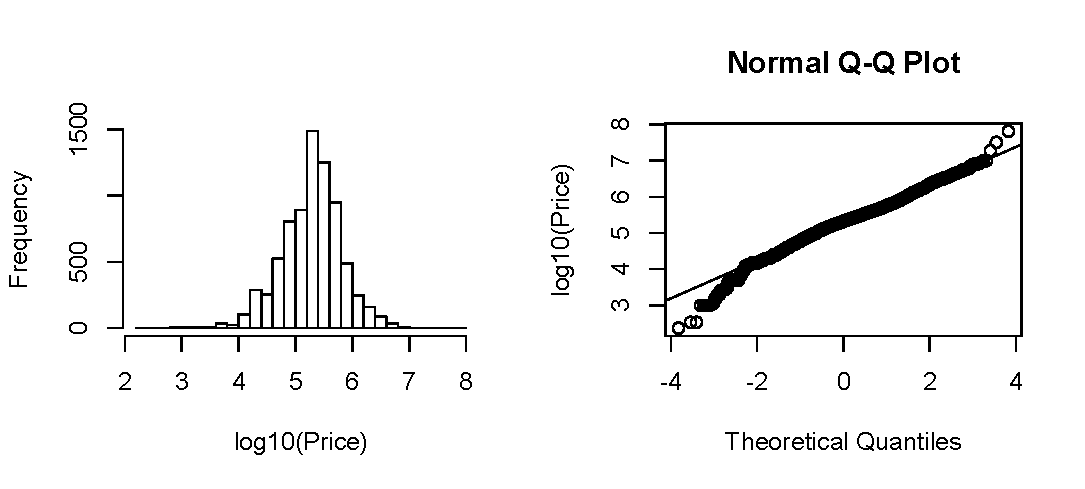
\includegraphics[width=5in]{figures/prices} }
 \vspace{0.2in}
 \end{figure}


 The listings that describe these properties are verbal, written in an
 idiosyncratic vernacular familiar only to those who are house hunting.  Some
 listings contain quantitative characteristics, but many do not.  The 
 following four listings are typical.  The initial value is the listed price.

 \begin{verbatim}
    $399000 Stunning skyline views like something from a postcard are yours
    with this large 2 bed, 2 bath loft in Dearborn Tower!  Detailed
    hrdwd floors throughout the unit compliment an open kitchen and
    spacious living-room and dining-room /w walk-in closet, steam
    shower and marble entry.  Parking available. 

    $13000 4 bedroom, 2 bath 2 story frame home. Property features a
    large kitchen, living-room and a full basement. This is a Fannie Mae
    Homepath property. 

    $65000 Great short sale opportunity...  Brick 2 flat with 3 bdrm
    each unit. 4 or more cars parking. Easy to show. 

    $29900 This 3 flat with all 3 bed units is truly a great
    investment!! This property also comes with a full attic that has
    the potential of a build-out-thats a possible 4 unit building in a 
    great area!!  Blocks from lake and transportation. Looking for a
    deal in todays market - here is the one!!! 
 \end{verbatim}

 \noindent
 Listings do not obey the grammatical rules of English.  Some authors write in
 sentences, others not, and a variety of abbreviations appear.  Punctuation varies from spartan to effusive (particularly exclamation marks),
 and the length of the listing runs from several words to a long paragraph.  The
 average listing has 73 words. The distribution of the lengths is right
 skewed; the shortest listing has 2 words whereas the longest has 568 words.
  This variation in the lengths of the descriptions suggests that modeling the
 prices from this text requires some form of weighting: we simply do not
 know much about properties with short descriptions.

  
 A natural approach for a statistician confronted with such data is to construct
 intuitively appealing regressors from the listings.  For example, one might
 conjecture that an agent has a lot more to say about an expensive property than
 one in need of repair.  Hence, the length of a listing 
 may be predictive of its price.  In a different vein, one can use regular
 expressions -- pattern matching -- to extract specific numerical data from the
 listings.  For example, the first listing indicates that this property has two
 bedrooms and two bathrooms.  A regular expression can be designed to extract
 numbers that precede the word ``bath'' from the listings.  Constructing such
 regular expressions, however, is a labor-intensive process that must be done on
 a case-by-case basis.  The patterns become complex because they must allow
 common abbreviations, such as ``bth'', ``bath'' and ``bthrm'' in order to match
 counts of the number of bathrooms.  Complexity aside, the greater problem with
 explicit pattern matching is that most listings omit these characteristics.
  The only numerical data common to every listing is the response, the
 advertised price.  For these listings, our regular expressions found that 6\%
 of the listings indicate the number of square feet, 26\% indicate the number of
 bathrooms, and 42\% give the number of bedrooms.  More complex regular
 expressions would likely find more matches, but the gains are likely to be few.
  As illustrated next, one faces a Type I/Type II trade-off.  Simple
 regular expressions miss some matches, but more aggressive expressions match
 inadvertently.


 The four scatterplots in Figure \ref{fig:parsed} summarize the marginal
 association between the log of prices and these constructed predictors,
 including the number of words in descriptions.  For listings with no match, we
 filled the missing values with the averages of the observed cases.  These
 appear as columns of gray points located at the mean of each variable on the $x$
 axis in Figure \ref{fig:parsed}.  The correlations between these variables and
 the log of the prices vary from moderate to nearly zero.  The length of the
 listing has the largest correlation with log prices ($r=0.40$). The frame that shows this association includes the fit of
 a fifth-order polynomial that recovers the evident nonlinearity of this
 association.  The nonlinearity is highly significant, but increases the amount
 of explained variation from 0.16 to only 0.20.  The improvement in fit is
 slight because most of the data lie within the linear range of the fit.
  Missing data has a large impact on the correlations with the other extracted
 features shown in Figure \ref{fig:parsed}.  The correlations for complete cases
 are 0.42 for the number of bathrooms, 0.26 for the log of the number of square
 feet, and 0.09 for the number of bedrooms.  If missing data are included, the
 correlations become much smaller (the second correlation shown in each frame).
  These plots also show several anomalies.  For example, the scatterplot of the
 log price on log length shows a cluster of 25 listings, all with exactly 265
 words (log 265=5.6).  These are not errors: All of these different properties
 were described in a common format by a government agency.  The scatterplot of
 the log of prices on the log of the square footage also shows a clear outlier;
 this outlier is a consequence of aggressive matching in a regular expression.
  A typo in a description (``has 1sfam'') led our regular expressions to find a
 property with 1 square foot.

 \begin{figure}
  \caption{ \label{fig:parsed} { \sl Extracted characteristics have moderate to
 slight positive association with the log of the prices. } Gray points in the
 figures identify cases that omit the explanatory variable; the first shown
 correlation in each frame uses only the observed data; the following smaller 
 value includes mean-filled listings. }
 
\centerline{
 \vspace{0.1in}
 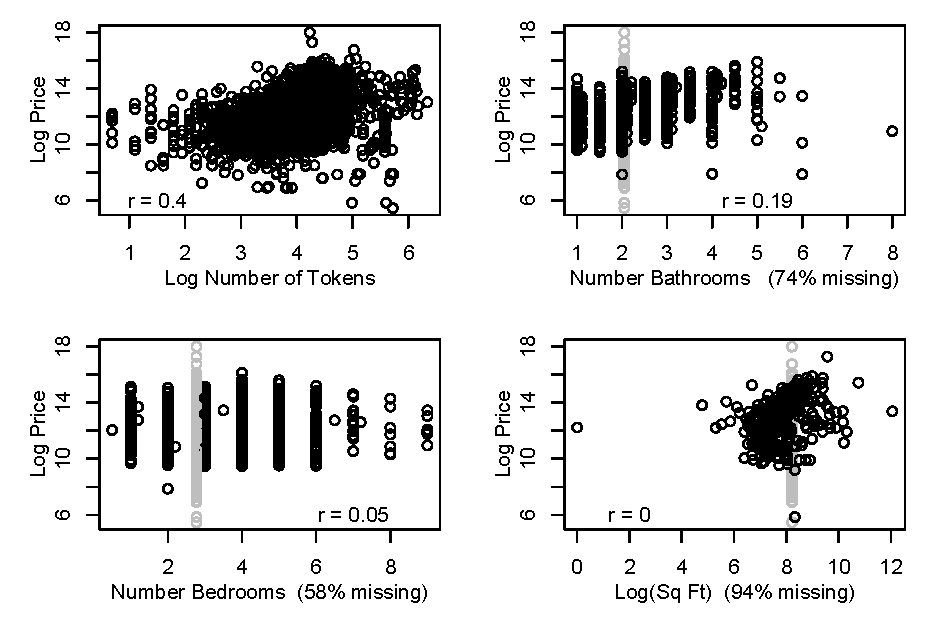
\includegraphics[width=5in]{figures/parsed} }
 \vspace{0.2in}
 \end{figure}


 Table \ref{tab:parsed} summarizes the fit of a regression of the log of price
 on predictors built from the four extracted features. The model includes a
 fifth degree polynomial in the log of the length of the description and missing
 data indicators.  These indicators are coded as 1 when the associated regular
 expression found a match and are coded as 0 otherwise.  Aside from the
 components of the polynomial, the features are not highly collinear, and the
 multiple regression echoes the marginal associations observed in Figure
 \ref{fig:parsed}.  Features related to the lengths of listings explain the most
 variation, followed by the number of bathrooms.  Unlike the marginal
 associations, the log of the number of square feet and its missing indicator
 are highly significant.  The missing indicators for bedrooms and bathrooms are
 not.  The model explains about one-fifth of the variation in prices;  adjusted R-squared $\ol{R}^2 = 0.232$ and, when adjusted for prediction, $\ars = 0.231$.  \ars adjusts $\R^2$ for predicting out-of-sample,

 
 \begin{table}[ht]
\caption{ \label{tab:parsed} {\sl OLS multiple regression of log prices on the
 parsed explanatory variables and  indicators of observed values.}}
\centering
\begin{tabular}{lrrrr}
  \hline
    Feature       & Estimate & Std. Error & t value & Pr($>$$|$t$|$) \\ 
  \hline
  Intercept       & 7.9985 & 0.4749 & 16.84 & 0.0000 \\ 
  log Tokens      & 39.0183 & 1.0945 & 35.65 & 0.0000 \\ 
  $(\mbox{log Tokens})^2$   & 1.0086 & 1.0642 & 0.95 & 0.3433 \\ 
  $(\mbox{log Tokens})^3$ & -18.2556 & 1.0612 & -17.20 & 0.0000 \\ 
  $(\mbox{log Tokens})^4$ & -4.8956 & 1.0594 & -4.62 & 0.0000 \\ 
  $(\mbox{log Tokens})^5$ & 7.9094 & 1.0584 & 7.47 & 0.0000 \\ 
  log Sq Feet     & 0.4039 & 0.0579 & 6.98 & 0.0000 \\ 
  Sq Feet obs     & 0.6254 & 0.0594 & 10.53 & 0.0000 \\ 
  Bedrooms        & 0.0080 & 0.0165 & 0.48 & 0.6299 \\ 
  Bedrooms obs    & -0.0084 & 0.0299 & -0.28 & 0.7783 \\ 
  Bathrooms       & 0.4015 & 0.0300 & 13.37 & 0.0000 \\ 
  Bathrooms obs   & -0.0199 & 0.0336 & -0.59 & 0.5537 \\ 
   \hline
   \multicolumn{5}{c}{$\ol{R}^2 = 0.232, \; s_e = 1.06$}\\
   \hline
\end{tabular}
\end{table}

 
 
 Had listings been composed in a consistent manner with a standardized set of
 characteristics, such constructive modeling would surely be more successful.
  Our goal here takes us in a different direction that, in contrast to this
 constructive approach, explores automatic methods that thrive in this
 unformatted, irregular context.  These methods are collectively known as {\em
 vector space models} in computational linguistics \citep[e.g.][]{turney10}.  A
 vector space model (VSM) characterizes each document as a point in some
 $p$-dimensional vector space (think \Rp).  VSMs originated in artificial
 intelligence and were adopted for text applications to construct a system for
 document retrieval known as latent semantic indexing \citep{deerwester88}.
  Latent semantic indexing clusters documents to enable a query to locate
 related items.  VSMs are closely related to techniques that statisticians will
 find familiar: principal components analysis (PCA) and canonical correlation
 analysis (CCA).  The underlying computational engine is a singular value
 decomposition (SVD), aided by random projections.  (The use of the SVD
 occasionally leads to VSMs being described as ``spectral algorithms'' which
 should not be confused with frequency domain methods for time series.)  There
 has been considerable debate as to how VSMs represent language; we leave to
 linguistics the task of explaining why such simple representations of text
 might capture deeper meaning \citep{deerwester90, landauer97, bullinaria07,
 turney10}.


 VSMs are commonly found in unsupervised applications such as clustering, but
 our application here finds that they are equally effective in supervised
 models.  In essence, each document becomes a point in \Rp, and these
 coordinates become regressors.  These regressors can be used alone or in
 combination with traditional variables, such as those obtained from a lexicon,
 regular expression, or semantic model.  The example of real estate listings
 illustrates the impact of various choices on the predictive accuracy.  For
 example, a regression using the automated features produced by a simple VSM
 explains over two-thirds of the variation in listed prices for real estate in
 Chicago.  The addition of several substantively derived variables adds little.
  Though we do not emphasize its use here, variable selection can be employed to
 reduce the ensemble of regressors without sacrificing predictive accuracy.  An application that models personality traits derived from Facebook
 messages appears in \citet{ungar13}.


 The remainder of this paper develops as follows.  The next section reviews
 latent semantic analysis (LSA) and uses this well-known method from
 computational linguistics to featurize text.  This method corresponds to
 principal components regression.  Section \ref{sec:cca} presents vector space
 models such as LSA from a novel perspective that emphasizes the statistical sense 
 of ``observations,'' samples drawn from a population.  LSA is seen to
 correspond to a CCA between words and the context of those words.  Various definitions of the
 context of a word allow one to construct many types of features.  Though
 embarrassingly simple to describe, it is more subtle to appreciate why a
 VSM works in regression.  Section \ref{sec:topicmodels} offers one
 explanation by relating VSMs to a type of topic model that reproduces many aspects of the real estate listings.  Section \ref{sec:cv} returns to regression models for real
 estate with a discussion of the use of variable selection methods ands use
 cross-validation to measure the success of methods and to compare several
 models.  Variable selection is particularly relevant if one chooses to search
 for nonlinear behavior.  We close in Section \ref{sec:disc} with a discussion
 and collection of future projects.



%--------------------------------------------------------------------------
\section{Featurizing with Latent Semantic Analysis}
\label{sec:lsa}
%--------------------------------------------------------------------------

 LSA is essentially a principle components analysis
 of a matrix whose elements count how often each word appears in a document (in our
 case, the frequency of words in a property listing).  Using these components as
 features in regression then amounts to a principle components regression.
  Quite a few details, however, need to be resolved in any application. For
 example, what is a word?  How should the data be scaled? 
 This section describes the relevant choices within
 the context of building a regression model for real estate prices.
 
 \subsection{ Tokenization }  % ------------------

 LSA begins by converting the source text into {\em word tokens}.  A word token
 is a sequence of one or more characters that represents an instance of a unique
 {\em word type}.  This conversion of text into tokens is known as tokenization.
  Tokenization requires making numerous, often subtle, choices.  For example, is
 the number ``735'' a word token?  Do the tokens ``state'' and ``State''
 represent the same word type?  Are ``room'' and ``rooms'' instances of the same word
 type?  To answer these questions, we adopt a standard, simple approach: we
 convert all text to lower case, distinguish punctuation characters as separate
 types, and replace instances of rare word types by a common token.  To
 illustrate some of the issues, consider the following listing:
 \begin{verbatim}
   Brick flat, 2 bdrm.  With two-car garage. \end{verbatim} 
 \noindent
 Separated into tokens, this text becomes a list of 10 tokens representing 9
 word types (angle brackets surround punctuation tokens)
 \begin{verbatim}
   {brick, flat, <,>, 2, bdrm, <.>, with, two-car, garage,<.> } \end{verbatim} 
 \noindent
 We leave embedded hyphens in place and do not correct spelling errors and
 typos.  Abbreviations remain as given.  References such as the texts by
 \citet{manning99} and \citet{jurafsky09} describe more elaborate choices, such
 as stemming and annotation, that can be incorporated into
 tokenization. \citet{turney10} give a concise overview.  Notice that
 tokenization only distinguishes word types, not  meaning or use
 (does not distinguish homographs).

  
 When applied to our data from Chicago, the 7,384 property listings contain
 536,485 word tokens representing 15,227 unique word types.  As usual in text,
 the most common word types occur frequently whereas most words appear
 infrequently.  More than half of these tokens appear only once or twice,
 providing little exposure to how the word is used.  We clustered these rare
 types into one category ($<$OOV$>$, for ``out of vocabulary''), resulting in a
 reduced vocabulary of $m = 5,707$ word types.  The most common word types are
 punctuation: `.'  occurs 40,227 times and `,' occurs 33,746 times.  Following
 these come the collection of seldom seen word types (OOV, 11,478), `and'
 (frequency 11,032), `!' (7,894) and `in' (7,418).  Figure \ref{fig:zipf} graphs
 the log of the frequency of these word types versus the log of their ranks.  It
 is common in text to find a linear trend with slope near 1 in this graph, the
 signature of a Zipf distribution \citep{zipf35, baayen02}.  In that case, the
 rank of a word type times its frequency would be constant.  Even though the
 text of real estate listings is not standard English, one expects to find
 counts resembling those produced by a power law \citep{clauset09}.  The shown
 line (with log-log slope -0.927) holds only for more common word types.  For
 less common words (here, outside the most common 500 words), the frequencies
 drop off more rapidly.  (This change in slope is also seen for words in
 Wikipedia.)


 \begin{figure}
 \caption{ \label{fig:zipf} { \sl The log of the frequency of word types in the
 listings for properties in Chicago is roughly linear in the log of the rank of
 the words.}  The shown line $\log \mbox{freq} = 10.9 - 0.93 \log \mbox{rank}$ 
 was fit to the most common words with ranks 1 through 500.  }

 \centerline{
 \vspace{0.1in}
 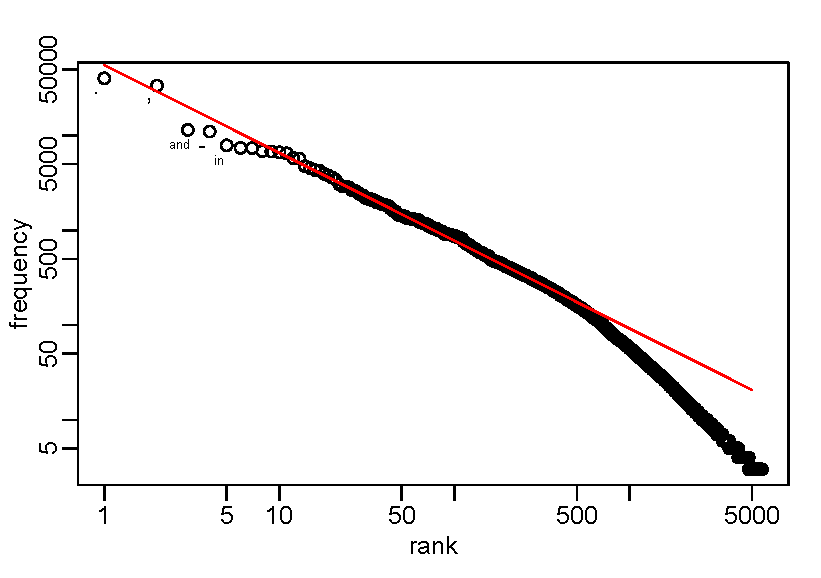
\includegraphics[width=3.5in]{figures/zipf} }
 \vspace{0.2in}
 \end{figure}


 Once the source text has been tokenized, we collect counts of how often each
 type appears within a listing.  These counts treat each listing as a ``bag of
 words,'' a multiset that does not distinguish the placement of words within a
 listing.  Permuting the words within a listing  produces the same
 counts.  Let $n$ denote the number of listings; we treat each listing as an observation
 in the usual sense.  Let $V$ denote the vocabulary, the set of
 $m$ distinct word types.  The $n \times m$ context-word matrix $W$ holds the counts of  
 these word types across the listings; $W_{ij}$ is the number of times word type $j$
 appears in the $i$th document.  (All vectors in our notation are column
 vectors.)  (The transpose of $W$, often called the term-document matrix, is common
 within computational linguistics. We follow the convention within statistics
 and arrange observations -- the listings -- as rows.)  The matrix
 $W$ is sparse: a small portion of the vocabulary appears in most documents. We assume that the columns of $W$ are sorted so that the first column holds the most frequent word type, the second column holds the second most frequent, and so forth.


\subsection{ Regressing on Word Types }  % ----------------------

Before turning to LSA, we fit models directly on the frequencies in $W$.  Because LSA constructs features that are linear combinations of the columns of $W$, all of the signal captured by LSA lies within $W$.  By regressing log prices directly on $W$, we can bound how much variation LSA can explain.  Our fits of log price on $W$ adjust for the lengths of the listings.  As shown in Figure \ref{fig:parsed}, the length of a listing is correlated with its price.  Keeping this polynomial in length in the regression implies that, for a word to be a significant predictor, its association with price must run deeper than its incremental contribution to the length.  Starting from this initial polynomial, we accumulated the $R^2$ statistic as first 3,000 columns of $W$ join the model.  The solid curves in Figure \ref{fig:cumr2} track $R^2$ as these frequencies are added in either decreasing (upper curve) or increasing (lower) frequency.  The gap between these curves shows that adding more frequent words first achieves a better fit with fewer variables. We also wanted to investigate the degree of collinearity within $W$.  PCA is useless if applied to orthogonal variables. The sparsity of $W$ produces small correlations between most columns of $W$, but colinearity emerges within larger collections.  For example, when adding features in order of decreasing frequency, 219 of these 3,000 word types were redundant and not added to the model.  To illustrate the effects of collinearity in regression, the dashed curve in Figure \ref{fig:parsed} shows the contribution to $R^2$ of words in order of decreasing frequency, but with the magnitude of the change in $R^2$ as if added in the other order.  For example, when added as the fourth feature, the count of OOV tokens boosts $R^2$ by about 0.02.  If added three steps ahead of the last variable, the frequency of OOV tokens adds much less to the fit, contributing only 0.0003 to  $R^2$.  

\begin{figure}
\caption{  \label{fig:cumr2}  
  {\sl Accumulated $R^2$ statistics of regression models with word frequencies added in order of decreasing (top solid black) or increasing (lower solid black) frequency.} The dashed curve shows the contributions having adjusted for subsequent words and illustrates the effects of collinearity among the word counts.}  
  \centerline{ 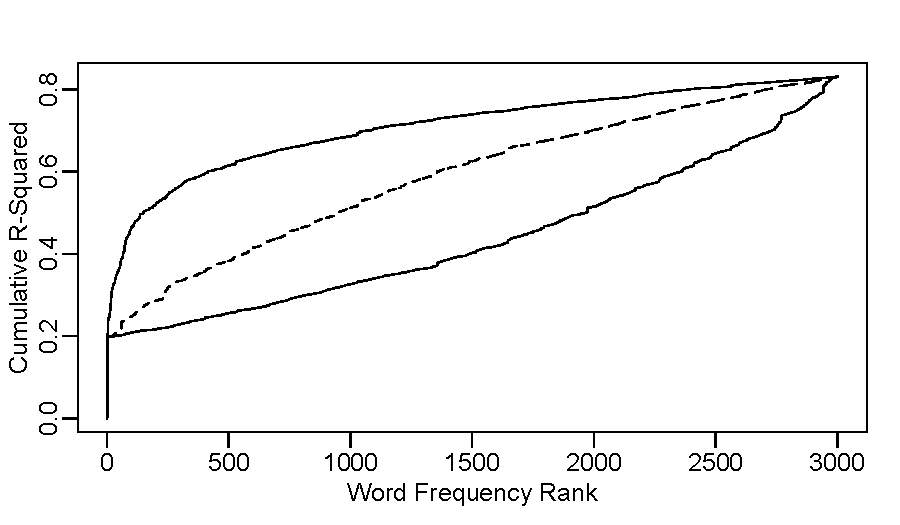
\includegraphics[width=4in]{figures/cumr2.pdf} }
\end{figure}


The slow growth of $R^2$ after the first hundred or so frequencies suggests that later features add too much noise to predictions and should not be in the model.  Even so, a model that simply adds the 3,000 most frequent words to the baseline polynomial provides a statistically significant improvement over the initial polynomial. Adding these words improves $R^2$ from 0.194 to 0.832, a highly significant increase.  Nonetheless, the resulting model is huge with many insignificant estimates.  One has numerous approaches to trimming its size, such as shrinkage or subset selection.  Because the word frequencies are correlated but easily ordered (by frequency), we use the corrected AIC statistic \citep{hurvich89}
\begin{equation}
    AIC_{c}(k) = n \log \frac{RSS(k)}{n} + \frac{n+k}{1-(k+2)/n} \;,
\end{equation}
where $k$ is the number of estimated parameters in the regression.  Rather than try to pick the best subset -- which would require a strong penalty against over fitting -- we use $AIC_c$ to pick the best stopping point in the single sequence of models determined by word frequency, much as one might pick the order of an autoregression.  Figure \ref{fig:aicwords} plots $AIC_c$ for the sequence of models obtained by adding words in order of decreasing frequency to the initial polynomial in log of the number of words.   The best fit  occurs with $k=1,089$ words, giving $R^2 =  0.705$ and $\ol{R}^2=0.654$. (The final model summarized in Figure \ref{fig:cumr2} with 3,000 words reaches $R^2 =  0.832, \, \ol{R}^2  0.719$.)  Residual plots show fat tails (consistent with the distribution of log prices in Figure \ref{fig:prices}), but no evidence of heteroscedasticity
 that might be anticipated due to the differences among the lengths of documents.

\begin{figure}
\caption{  \label{fig:aic}  
  {\sl Corrected AIC for two regression models: one adds words in order of decreasing frequency (dashed) and a second that adds LSA components (solid).}  Vertical gray segments mark the positions of the minimum $AIC_c$.}
  \centerline{ 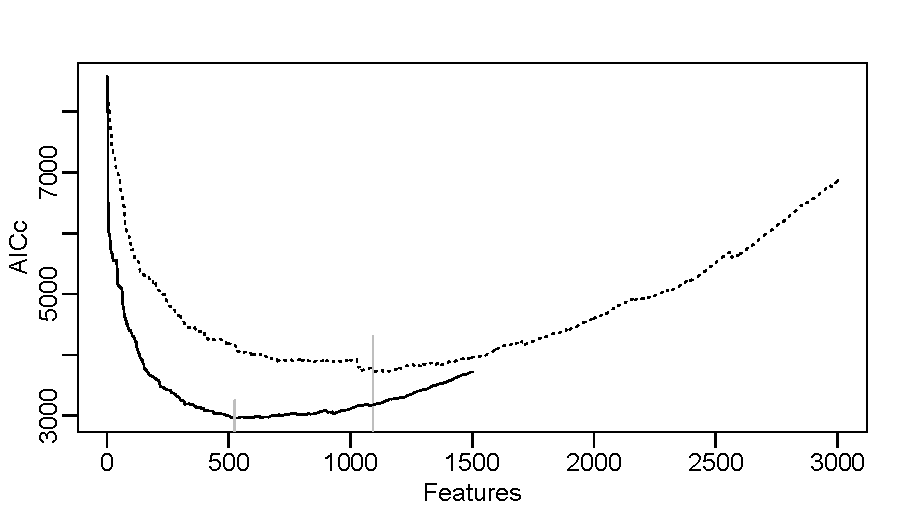
\includegraphics[width=4in]{figures/aic.pdf} }
\end{figure}


\begin{figure}
\caption{  \label{fig:aictstats}  
  {\sl Absolute $t$-statistics from the regression of log prices on words for the model selected by $AIC_c$.}  In the left panel, the horizontal black line is $\ev |Z|$ for $Z \sim N(0,1)$,  the higher dashed line is the Bonferroni threshold, and the red curve is a loess smooth of $|t|$.  In the right panel, the red line is fit to the smallest 20\% of the $|t|$-statistics, producing the shown slope.}
  \centerline{ 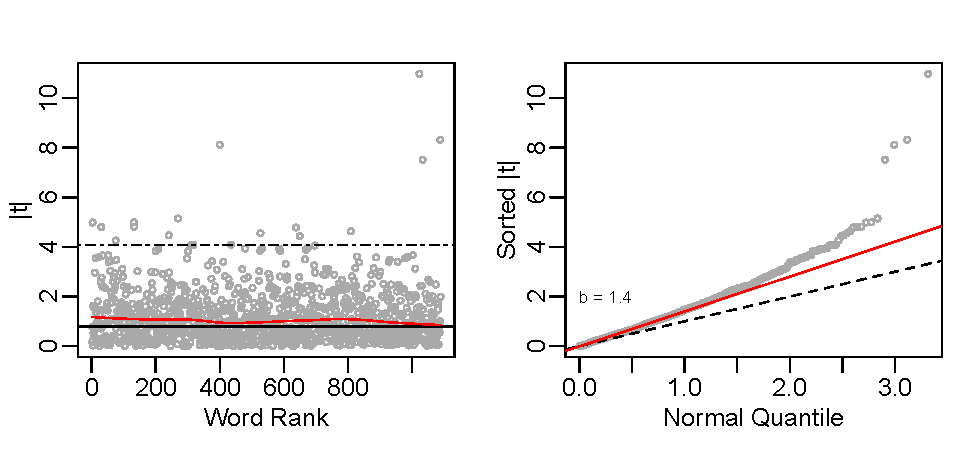
\includegraphics[width=4in]{figures/aictstats.pdf} }
\end{figure}

 
Although the model selected by $AIC_c$ explains a great deal of variation in prices, the signal remains diffusely spread over the words.  Few estimates stand out, leaving substantial signal embedded in the background.   Figure \ref{fig:aictstats} summarizes the t-statistics in this fit. The left panel of the figure graphs $|t|$ for the words in order of decreasing frequency.  The solid horizontal black line is the expected value of the absolute value of a standard normal, $\sqrt{2/\pi}$. The dashed horizontal line is the Bonferroni threshold $\Phi^{-1}(1-0.025/1089) \approx 4.08$.  Between these, the almost flat red curve is the loess smooth of  $|t|$; the average $|t|$ is only slightly larger than one expects for a model with no signal.   Coefficients of only 16 words exceed the Bonferroni threshold.  For example,
 the coefficient for the word ``vacant'' has $t=-8.1$; not  surprisingly, the
 addition of this word to a listing lowers the expected price.  In
 contrast, the presence of additional out-of-vocabulary words
 suggest with higher than average prices ($t=5.0$).   Though these stand out, these few words explain only a small portion of the fit.  A regression restricted to the 16 words that exceed the Bonferroni bound obtains
 $\ol{R}^2 = 0.236$. The half-normal plot in the right panel of
 Figure \ref{fig:aictstats} confirms the diffuse signal: the fitted $t$-statistics are inconsistent with noise, but not by much.  The dashed line in the half-normal plot is the diagonal; the red
 line is a  regression fit to the smallest 20\% of the $|t|$-statistics.  For a sample from a standard normal distribution, the slope should be 1.  The slope of these estimates is significantly larger, but clearly the signal is
 widely spread.   
   

 \subsection{ Regressions using LSA }  % ------------------

The use of LSA to create features for regression models essentially reproduces principal components regression.  The only differences are the absence of centering and the variety of approaches for weighting counts prior to constructing the principal components. For example, one might choose to stabilize the variance of the counts.  Define ${W}^{*}$ to be the $n \times m$ matrix with elements ${W}^{*}_{ij} = W_{ij}/\sqrt{n_i}$ with $n_i = \sum_j W_{ij}$ counting the number of word tokens in the $i$th document.  Were tokens within listings random samples from
 a multinomial distribution with probabilities $p_{1:m}$ across the word types, then $\Var({W}^{*}_{ij}) = p_j(1-\sum_{k\ne j} p_k)$, without dependence on the number of words in the listing. Similarly, we can define $\tilde{W}$ with elements $\tilde{W}_{ij} = W_{ij}/\sqrt{m_j}$ with $m_j = \sum_i W_{ij}$ counting the number of tokens of word type $j$. This scheme down-weights the most common word types, which is sensible given that the presence of rare  OOV words is a significant indicator of higher priced listings.  Similarly, the popular method known as term frequency-inverse document frequency (TF-IDF) also emphasizes less common word types, but counts the number of documents in which a word appears rather than its frequency overall.  In the simplest version of TF-IDF,  let $d_j = \sum _i\one{W_{ij} >
 0}$ count the number of listings in which word type $j$ appears and replace $W_{ij}$ by
 $W_{ij} \log(n/d_j)$.  For example, if the word type ``.'' appears in
 every listing, then $\log n/d_j = 0$, removing this ubiquitous
 type from the construction of principal components.
 \citet{turney10} provides further motivation for these and other weightings used in LSA.
  In our application, we use $\tilde{W}$ because of  its ability to recover structure for data generated by in the probability model described in Section {xx}.  In the expressions that follow, we generically use $W$ to stand for any of these weighted versions of the counts.
 
 
 We compute the leading principal components of $W$ by using random projections that
 closely approximate the truncated SVD of $W$.  Denote the SVD of the context-word matrix $W$ by
 \begin{equation}
       W = U D V' = \sum _{i=1}^{\min(m,n)} \la_i u_i v_i' \;,
 \end{equation}
 where $U = [u_1,\ldots,u_n]$ and $V=[v_1,\ldots,v_m]$ are orthonormal, and $D = \mbox{diag}(\la_i)$ is a $n \times m$ diagonal matrix,
 with the singular values $\la_1 \ge \la_2 \ge \cdots \ge \la_{\min(m,n)}$ along the diagonal.  The columns of $U$ are the eigenvectors of $X'X$ (the sought principal components,
 or left singular vectors), and the columns of $V$ are
 the eigenvectors of $XX'$.  The truncated, or thin, SVD zeros all but the
 largest, say, $k$ singular values and produces an approximate
 factorization of $W$ that we denote
 \begin{equation}
       W_k \approx U_k D_k V_k' = \sum _{i=1}^k \la_i u_i v_i' \;,
 \label{eq:Wk}
 \end{equation}
 $U_k$ and $V_k$ hold the first $k$ columns of $U$ and $V$, respectively, and $D_k$ is the corresponding leading portion of $D$.  Because of the size of $W$, the computation
 of $W_k$ can be very slow.  
 It is worthwhile to take note of two properties of these calculations that are
 important in practice.  First, one needs to take advantage of sparsity in  $W$ to reduce memory usage and to increase the speed of
 computing matrix products.  Second, even leveraging sparsity, the computation of the SVD of a large
 matrix can be quite slow. 
  To speed this calculation, we exploit random projection algorithms defined and
 analyzed in \citet{tropp10}.

Since we only require the portion of the range of $W$ captured by $U_k$, however, we can 
 exploit the algorithms based on random projection \citep{tropp10}.  
 
 
 Suppose in the ideal case that $W$ essentially has rank $k$ in the sense that $\la_k \gg 0$ and $\la_{k+1} \approx 0$.  Let $\ell$
 denote an integer slightly larger than $k$ \citep[see][for the
 details]{tropp10}.   Form an $m \times \ell$ matrix $\Omega_{\ell}$ with random
 elements $\Omega_{ij} \sim N(0,1)$, independently, and compute the product
 $A_{\ell} = (W W')^q W \Omega_{\ell}$ for small $q$.  (We set $q = 4$.)  The initial multiplication of $W$ by $\Omega_\ell$ reduces the number of columns
 from $m$ to $\ell$;  subsequent multiplication by $W W'$ improves the
 approximation, resembling the power method for finding eigenvalues. $(W W')^q W$ has the same singular vectors as $W$, but its singular values are $\la_j^{q+1}$, which typically increases the spread between $\la_k$ and $\la_{k+1}$.   The matrix product that defines $A_\ell$ can be done quickly by exploiting
 the sparsity of $W$.  Let $Q_{\ell}$ denote an orthonormal basis for the range of $A_{\ell}$, such as through a QR factorization $A_\ell = Q_\ell R_\ell$.  At the end of these steps, \citet{tropp10} shows that we obtain a low-rank factorization of $W$ in the sense that 
 \begin{equation}
   \norm{W - Q_{\ell} Q_\ell' W} \le  \left(1+11 \sqrt{\ell} \min(m,n)\right) \la_{k+1}
\label{tropp}
 \end{equation}
 with high probability.  $\norm{\cdot}$ denotes the spectral norm of a matrix.
 To obtain the SVD of $W$, we need only compute the SVD of the much smaller matrix $C_\ell = Q_\ell'W$.  Write the SVD of $C_\ell$ as $C_\ell = U_c D_c V_c'$.  If we plug this expression into the low-rank representation for $W$, we obtain $W \approx Q_\ell U_c D_c V_c'$. The first $k$ columns of $Q_\ell U_c$ approximate  $U_k$.  \citet{tropp10}
 provides a thorough analysis this algorithm, so we
 illustrate its performance within the context of the analysis of real estate listings.


 The spectrum of the context-word matrix $W$ lacks the distinct gap that would suggest the rank needed to obtain an accurate low-rank approximation.  Figure \ref{fig:spectrum} graphs the singular values of $\tilde{W}$ on a log scale. (Other scalings of $W$ produce similar spectra.)  After the first few elements, the singular values fall off steadily, without the sort of gap described for the idealized case.  The absence of a clear rank complicates the choice of how many components to use in a regression, so once again we use $AIC_c$.  In this case, we order the features by singular value.

 \begin{figure}
 \caption{ 
 	\label{fig:spectrum}
	{\sl The spectrum of the document-term matrix $\tilde{W}$ decays relatively slowly 
	      after the initial sharp drop. }}

 \centerline{
 \vspace{0.1in}
 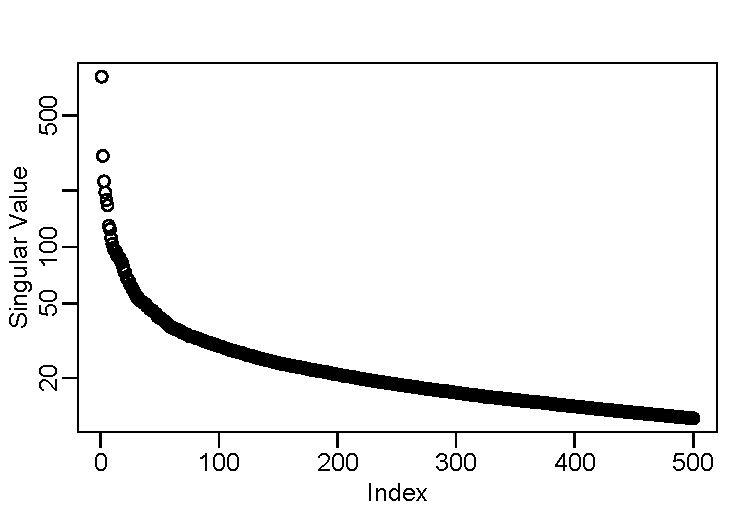
\includegraphics[width=3.5in]{figures/spectrum} }
 \vspace{0.2in}
 \end{figure}
   
The conversion of words into LSA components produces a qualitative change in the structure of the $t$-statistics.  Figure \ref{fig:lsatstats} summarizes (in the same format as Figure \ref{fig:aictstats}) the $|t|$-statistics from a regression using the first 1,000 LSA component features. (As with words, the model includes a polynomial in document length.) Unlike the regression on frequencies of word types, the average magnitude of the $|t|$-statistics in this regression decline roughly monotonically, with the most significant effects present in the initial components and gradually falling off. Some signal remains in the smaller components (the slope in the half-normal plot is 1.8), but sorting based on singular value is far more useful than sorting on word frequency.  The fitted model obtains $R^2 = 0.718$ with $\ol{R}^2 =  0.674$, compared to $\ol{R}^2 = 0.654$ for the previous regression on 1,089 words.  Consequently, with more signal in the earlier components, $AIC_c$ finds a more predictive model with fewer coefficients.  The sequence of $AIC_c$ statistics for this model lies well below that for the regression on word frequencies in Figure \ref{fig:aic}.  $AICc$ selects the model that uses 523 LSA components, obtaining $R^2 = 0.677$ and $\ol{R}^2  = 0.652$.  

[ Though the $t$-statistics are more conveniently positioned by LSA than those in the regression directly on word frequencies, these models share similar explanatory power.  ]
 
\begin{figure}
\caption{  \label{fig:lsatstats}  
  {\sl Absolute $t$-statistics from the regression of log prices on the first 1,000 LSA components with column weighting.}  }
  \centerline{ 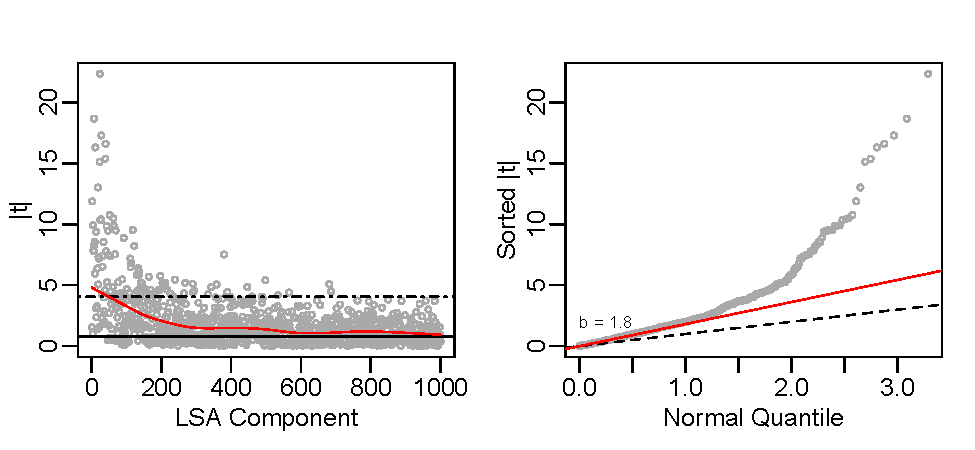
\includegraphics[width=5in]{figures/lsatstats.pdf} }
\end{figure}



 
%--------------------------------------------------------------------------
\section{A Numerical Representation and More Features}
\label{sec:cca}
%--------------------------------------------------------------------------

We can recast the frequencies in the document-word matrix $W$ as covariances between two types of indicator variables. This alternative perspective provides a basis for creating a wide range of features from text.  The key notion that distinguishes this alternative perspective is to think of text data as defining a large binary matrix.  Recall that we have $n$ documents, with $n_i$ word tokens in document $i$ chosen from a vocabulary of $m$ word types.  Begin by concatenating the word tokens of every document (real estate listing) into a list, say
\begin{equation*}
   \ell = \underbrace{w_{11},\,w_{12},\ldots,w_{1n_1}}_{\mbox{doc 1}},\,
            \underbrace{w_{21},\ldots,w_{2n_2}}_{\mbox{doc 2}}, \,
            \ldots, \underbrace{w_{n1},\ldots,w_{n_nn}}_{\mbox{doc }n},
\end{equation*}
with length $N = \sum n_i$ word tokens.  From this sequence, define the $N \times m$ indicator matrix $X$ for which $X_{ij} = 1$ if the $i$th word token in $\ell$ is of type $j$.  $X$ is large a very sparse, with a single 1 in each row, 
\begin{equation}
  X =   \left( \rule{0em}{8em} \right.
  \begin{array}{cccccccc}
            \mbox{\scriptsize $w_1$} &
            \mbox{\scriptsize $w_2$} &
            \mbox{\scriptsize $w_3$} &
            \mbox{\scriptsize $w_4$} &
            \mbox{\scriptsize $w_5$} &
            \mbox{\scriptsize $w_6$} &   \cdots &
            \mbox{\scriptsize $w_m$}  \cr
            0  & 0 & 1 & 0 & 0 & 0 & \cdots & 0 \cr
            0  & 0  & 0 & 0 & 1 & 0 & \cdots & 0 \cr
             &&&  \vdots &&&&                                 \cr
            0  & 1  & 0 & 0 & 0 & 0 & \cdots & 0 \cr \hline
            0  & 0 & 0 & 0 & 1 & 0 & \cdots & 0 \cr
              &&&  \vdots &&&&                                 \cr
            1  & 0 & 0 & 0 & 0 & 0 & \cdots & 0 \cr \hline
              &&&  \vdots &&&\ddots&                                 \cr
              \\
           \end{array}
        \left. \rule{0em}{8em} \right)
        \;.
\end{equation}
This matrix {\em is} the text data.  Given this numerical representation, we are back in familiar territory.  The data are numerical rather than text.  To obtain the counts used in LSA, define an $N \times n$ context matrix $L$  that identifies the documents,
\begin{equation}
  L =  \left(  
           \begin{array}{ccccc}
            1  & 0 & 0 & \cdots & 0 \cr
            1  & 0 & 0 & \cdots & 0 \cr
             &&  \vdots &&                       \cr
            1 & 0 &  0 & \cdots & 0 \cr \hline
            0 & 1 & 0  & \cdots & 0 \cr
              &&  \vdots &&                        \cr
            0 & 1& 0 & \cdots & 0 \cr \hline
              &&  \vdots  &\ddots&             \cr
            0 & 0& 0 & \cdots & 1 \cr \hline        
           \end{array}
         \right) = I_n \otimes \one{n_i}  \;,
\end{equation}
where $\one{n}$ denotes a column vector of $n$ 1s. (Here we abuse the usual Kronecker product and allow the constant vectors to have unequal length.)  The document-word matrix $W$ is then $N-1$ times the observed covariance matrix between $X$ and $L$,
\begin{equation*}
   W = (N-1) \cov(L,X) = L'X  \;.
\end{equation*}
Once we think of $W$ as a covariance matrix, it becomes natural to associate LSA with canonical correlation analysis (CCA) rather than PCA.  In order for the SVD of $W$ to produce canonical vectors, however, we have to standardize the columns of $L$ and $X$.  Let $S_L = L'L/(N-1) = \mbox{diag}(n_i)$ and $S_X = X'X/(N-1)$ denote the uncentered covariance matrices.  \ras{Why not centered?}  The SVD of $S_L^{-1/2} W S_X^{-1/2}$ then yields the canonical correlations and vectors. \ras{cite Dean and Sham}  Standardizing $L$ is easy because its columns are orthogonal (when uncentered), but those of $X$ are not.  Commonly, then, one uses the approximation $\widetilde{S}_X = \mbox{diag}(m_j)$, with $m_j$ counting the number of tokens of word type $j$.  As explained in Section \ref{sec:topic}, we use partial standardization and work with $\widetilde{W} =X \widetilde{S}_X^{-1/2}$.


 Now that we have a numerical representation of text, a variety of other featurizations become apparent.  The sequential nature of the rows of $X$ suggest ideas from time series analysis, particularly lags.  For instance, we might find interesting patterns in the association between the word type that appears next to each other in positions $i-1$ and $i$.  Let $X_{-1}$ denote the lag of $X$ obtained by inserting a leading row of zeros and removing the final row.  Rather than use documents to define context, we use the previous word.  The counts that produce the covariance between this context and the word at location $i$ define a bigram matrix $B$,
 \begin{equation}
   B = X_{-1}' X
\end{equation}
Using the prior word to define a context removes the role of documents and treats the list $\ell$ as a stochastic process.  Where $W$ uses the wide context defined by the extent of documents in the text, $B$ uses the narrow, very local context defined by the prior word. Notice that $W$ ignores word placement (sequencing) within a document (treating a document as a bag of words); in contrast $B$ combines the documents and relies only on the sequence of word tokens. The wide context afforded by a document hints that $W$ emphasizes semantic similarity, whereas the narrow context of adjacency suggests $B$ emphasizes syntax.  Either approach can be effective.

 
 As in LSA, we obtain features from the leading singular vectors of $B$.  Again, random projection speeds this calculation.  Let $\widetilde{U}_{B,k}$ denote the leading $k$ singular vectors obtained from the approximate SVD of the standardized bigram matrix $S_X^{-1/2} B S_X^{-1/2}$.  The columns of $\widetilde{U}_{B,k}$ are sometimes called ``eigenwords'' because of the way in which they form directions in word space \ras{cite lyle or someone using this name}.  Each row of $\widetilde{U}_{B,k}$ represents a word type as a point in $\R^k$.   To build features for regression, we simply locate each document at the average position of its words, $(I_n \otimes \one{n_i}/n_i)'\widetilde{U}_{B,k}$. 


%--------------------------------------------------------------------------
\section{Predicting Prices of Real Estate}
%--------------------------------------------------------------------------


 The next model uses regressors created from the SVD of the document/word
 count matrix $W$ defined in equation \eqn{svdW}.  We retained $k_W = 100,\, 200, \, \ldots, 500$ singular vectors of $W$.   Our analysis suggests each of these collections of singular vectors both retains too many insignificant features while at the same time omits others that are predictive.  Broadly speaking, the leading singular vectors (those with larger singular values) are more predictive than subsequent singular vectors.  That said, not all of the leading vectors are statistically significant nor do all of the later singular vectors have coefficients near zero.   As a result, variable selection from a yet larger collection of singular vectors may provide a better fit, a task we defer to Section \ref{sec:cv}.  
 
 \citet[do CCA before regression][]{fosterkakade07}

Each collection of singular vectors explains more variation than the simple model derived from several parsed words, but none find all of the signal captured by the larger collection of 2,000 word indicators.  A regression of log prices on the 100 leading singular vectors attains $\ol{R}^2 = 0.49$, more than twice that of the model with parsed variables.  Adding more singular vectors produces statistically significant, though diminishing improvements.  The collection of 500 singular vectors of $W$ produces $\ol{R}^2 = 0.61$, which is less than the $\ol{R}^2 = 0.68$ derived from individual word counts.  Table \ref{tab:regrW}  shows several of the estimated coefficients and summarizes the overall fits of these models.  As often seen in principal components regression, the statistical significance of the singular vectors is not monotonic in the order of the singular vectors. That said, the leading singular vectors tend to be more relevant than those that follow. Figure \ref{fig:svdregr} summarizes the significance of the estimated coefficients in the same fashion as Figure \ref{fig:regrInd} with a plot of the absolute $t$-statistics and a half-normal plot. Most of the main leading singular vectors are significant, with an increasing proportion of insignificant variables as the position in the decomposition increases.  In comparison to the significance for the coefficients of the word indicators, these singular vectors by-and-large are more consistently predictive with less noise.  The slope of the fit in the half-normal plot (using the least significant 200 estimates) is 2.9.  Residual analysis again finds fat tails with only a hint of heteroscedasticity.
 
 
 Not only can one continue to add further singular vectors, one can also consider nonlinearities in the form of interactions among these singular vectors.  The addition of interactions improves the fit of this model immensely by taking advantage of nonlinearities (\ie, synergies among the eigenword structure).  For example, a regression using just the first 20 singular vectors of $W$ obtains $\ol{R}^2 = 0.31$.  Adding interactions among these (an additional 190 explanatory variables since no powers are added) improves the fit significantly to $\ol{R}^2 = 0.41$.  Fitting models with interactions drawn from a larger collection of features more generally requires some form of selection or regularization.  We pursue this further in Section \ref{sec:cv}.
 

 \begin{table}
 \caption{ \label{tab:regrW} {\sl Multiple regression of log prices on
  singular vectors of the document/word count matrix $W$.}  The first table shows estimated coefficients for first 10 and last 3 singular vectors with $k_w = 500$.  }

\begin{center}
\begin{tabular}{rrrrr}
  \hline
 & Estimate & Std. Error & t value & Pr($>$$|$t$|$) \\ 
  \hline
  D1 & -62.0847 & 2.4891 & -24.94 & 0.0000 \\ 
  D2 & -7.6494 & 0.9373 & -8.16 & 0.0000 \\ 
  D3 & -12.5468 & 0.7558 & -16.60 & 0.0000 \\ 
  D4 & 10.4948 & 0.8262 & 12.70 & 0.0000 \\ 
  D5 & -0.8683 & 0.7645 & -1.14 & 0.2561 \\ 
  D6 & 7.6848 & 0.8036 & 9.56 & 0.0000 \\ 
  D7 & -17.8753 & 0.7547 & -23.69 & 0.0000 \\ 
  D8 & 18.8346 & 0.7577 & 24.86 & 0.0000 \\ 
  D9 & 3.9515 & 0.7540 & 5.24 & 0.0000 \\ 
  D10 & 4.0974 & 0.7521 & 5.45 & 0.0000 \\  
  $\vdots$ & & & & \\
  D498 & 1.2327 & 0.7516 & 1.64 & 0.1010 \\ 
  D499 & 1.3265 & 0.7516 & 1.76 & 0.0776 \\ 
  D500 & 2.5296 & 0.7516 & 3.37 & 0.0008 \\ 
   \hline
\end{tabular}
\end{center}


\begin{center}
\begin{tabular}{ccccc}
	$k_w$   & Residual SD & $F$ & $R^2$  & $\ol{R}^2$  \cr
	100       &  0.863   & 72.1  & 0.496  & 0.489  \cr
	200       &  0.810   & 45.9  & 0.561  & 0.549  \cr
	300       &  0.778   & 35.5  & 0.601  & 0.584  \cr
	400       &  0.765   & 28.5  & 0.620  & 0.598  \cr
	500       &  0.752   & 24.3  & 0.638  & 0.612
\end{tabular}
\end{center}
\end{table}


 The third regression uses features derived from the SVD of the bigram matrix
 $B$ defined in \eqn{svdB}.  For this analysis, we retained $k_B=100, 200, \ldots, 500$ left and right singular vectors ($k_B$ columns in each of $U_B$ and $V_B$) and for each computed the associated matrix of correlations $C$.  With $2 \, k_B = 1,000$ left and right singular vectors, the largest $\ol{R}^2 = 0.66$, slightly more than the 0.61 obtained using the 500 singular vectors defined from $W$.  Table \ref{tab:regrB} summarizes these fits.  Using correlations from either the left or right singular vectors alone (derived from either $U_B$ or $V_B$) explains significantly less variation; for example, a regression on 500 correlation vectors derived from  $U_B$ alone  produces $\ol{R}^2 = 0.61$ (about the same as obtained from the 500 singular vectors of $W$). The use of the left and right singular vectors produces collinearity among the explanatory variables.  A consequence of this collinearity is a large number of insignificant regressors in the fitted model.  Figure \ref{fig:svdregr}(b) shows the p-values generated by the 500 singular vectors of correlations.  Compared to the singular vectors derived from $W$ shown in Figure \ref{fig:svdregr}(a), these regressors have more diffuse signal.  The slope in the half-normal plot (again, derived from the least significant 200 estimates) is 2 (compared to 2.9 for the regressors derived from $W$).  Also, the trend in the half-normal plot is concave rather than convex; the most significant variables are less significant than anticipated by the signal in the smaller estimates.

 \begin{figure}
 \caption{ \label{fig:svdregr} { \sl T-statistics of the singular value regressors
 for (a) the singular vectors of $W$ and (b) the left and right singular vectors
 of $B$.}}
 \vspace{0.1in}
 % \centerline{  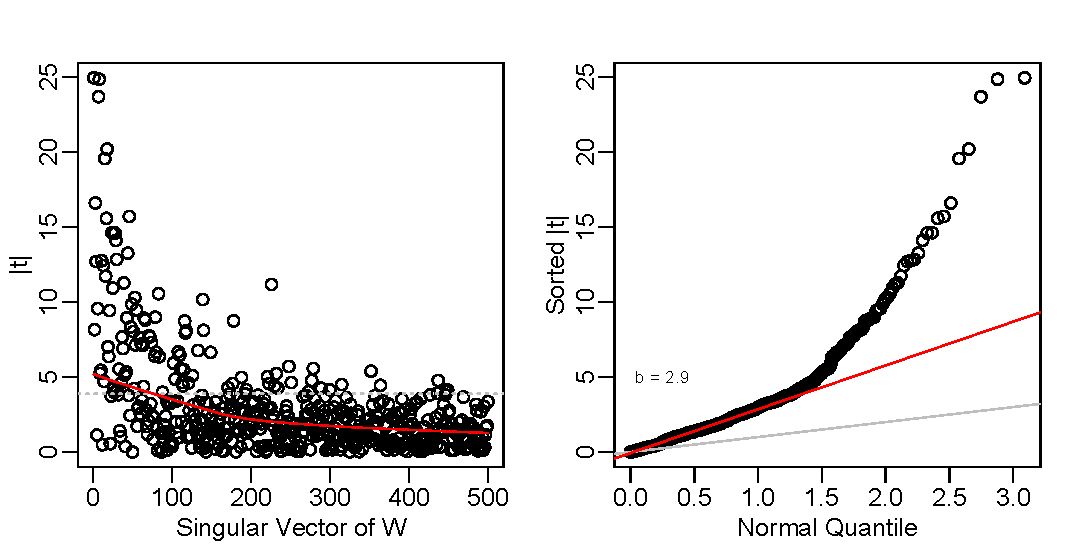
\includegraphics[width=6in]{figures/regrW}  }
 \centerline{  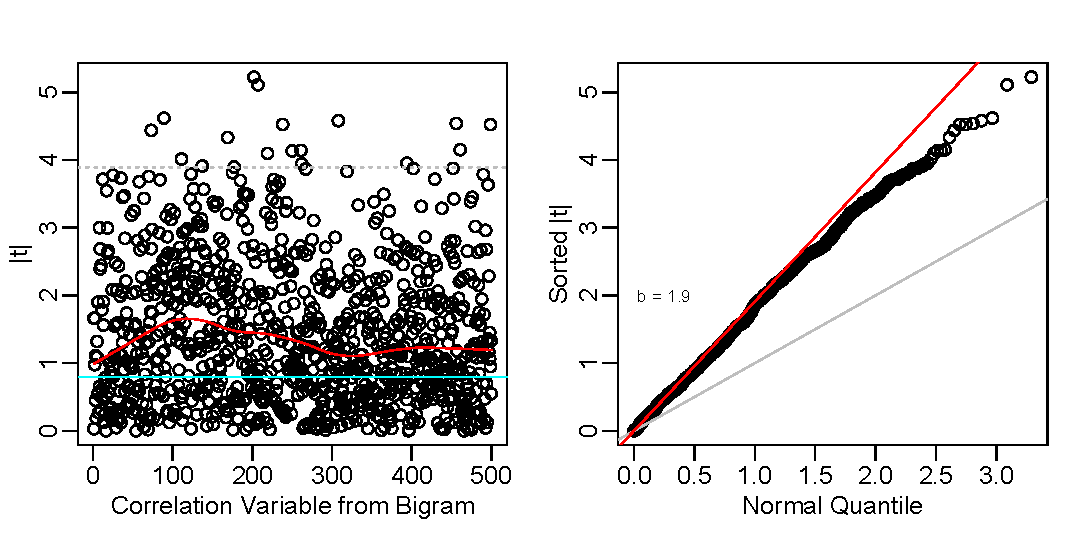
\includegraphics[width=6in]{figures/regrB}  }
 \end{figure}


\begin{table}
\caption{ \label{tab:regrB} {\sl Multiple regression of log prices on regressors derived from the bigram matrix $B$.}  Each regression uses correlations derived from $k_B$ left and $k_B$ right singular vectors.  }
\begin{center}
\begin{tabular}{ccccc}
	$2\,k_B$   & Residual SD &  $F$ & $R^2$  & $\ol{R}^2$  \cr
	200           &  0.842           &  40.0 &  0.527 &  0.514 \cr
	400           &  0.779           &  26.8 &  0.605 &  0.583 \cr
	600           &  0.750           &  20.6 &  0.645 &  0.614 \cr
	800           &  0.724           &  17.4 &  0.679 &  0.640 \cr
	1000         &  0.704           &  15.3 &  0.705 &  0.660
\end{tabular}
\end{center}
\end{table}


We can concentrate more of the regression signal into the leading components by using canonical correlation analysis.  Figure \ref{fig:cca} shows the canonical correlations between  $C_l$ and $C_r$.  The correlations remain close to 1 for about the first 100 or so canonical variables.  Rather than use the columns of $C_l$ as regressors, we can use the canonical variables from this analysis.  Figure \ref{fig:regrBcca} summarizes the estimates using the 500 predictors.  The regression signal is now much more concentrated in the leading canonical variables, resembling the structure found by LSA (Figure \ref{fig:regrW}).  The overall fit, of course, matches that obtained by using $C_l$ since the canonical vectors are linear transformations of $C_l$.  We conjecture that CCA has this effect because, under the simple topic model introduced in Section \ref{sec:model} that follows, the left and right singular vectors of $B$ measure essentially the same thing and aligning these via CCA produces a better measure of that common structure.  This alignment, however, removes the distinction due to word order that the bigram matrix reveals.  It may be the case that in this relatively small example (\ie, relatively few documents) we lack enough text to exploit asymmetry in the use of words.
 
 
 \begin{figure}
 \caption{ \label{fig:cca} { \sl Canonical correlations between the 500 columns of $C_l$ and $C_r$.}}

 \centerline{
 \vspace{0.1in}
 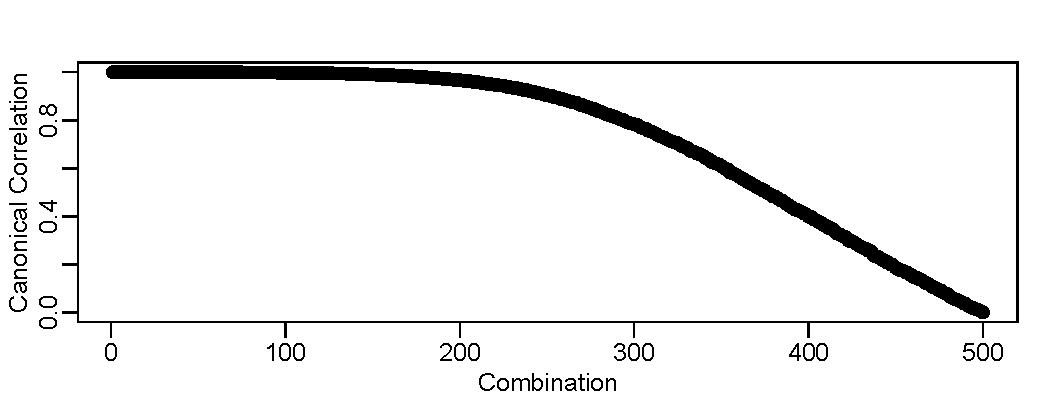
\includegraphics[width=3in]{figures/cca}  }
 \vspace{0.2in}
 \end{figure}


 \begin{figure}
 \caption{ \label{fig:regrBcca} { \sl Canonical variables from the analysis of the dependence between $C_l$ and $C_r$ concentrate more signal into the leading regressors.}}

 \centerline{
 \vspace{0.1in}
 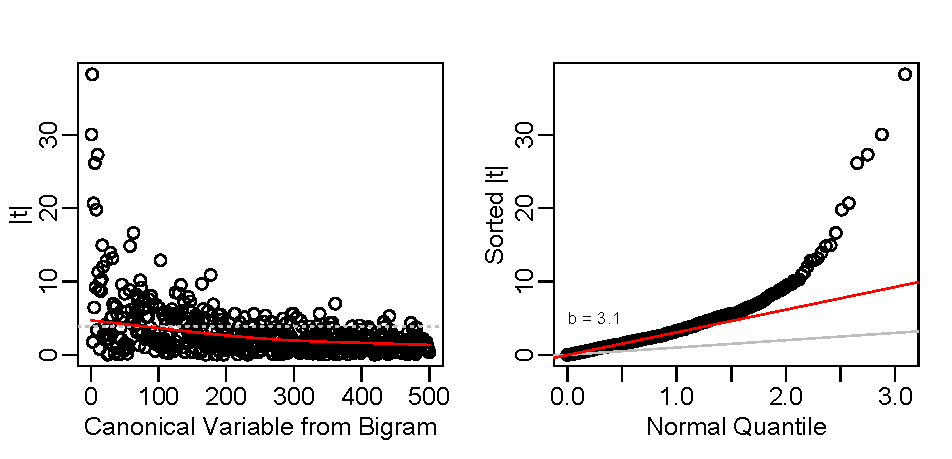
\includegraphics[width=5in]{figures/regrBcca}  }
 \vspace{0.2in}
 \end{figure}


How well does combining both sets of variables perform?  To find out, we start with the variables from the LSA, the singular vectors of $W$.   The regression on the 500 singular vectors in $U_W$ explains $\ol{R}^2 = 0.612$ of the variation in log prices.  Adding the information from 500 more columns in $C_l$ boosts the total to $\ol{R}^2 = 0.679$.  Adding the remaining variation from $C_r$ raises the total slightly (albeit significantly) to $\ol{R}^2 = 0.703$. Interestingly,  the original parsed variables (Table \ref{tab:parsed}) offer ever so slightly more predictive power. The improvement only adds 0.003 to $\ol{R}^2$, but this is highly significant ($F$=12.1).


%--------------------------------------------------------------------------
\section{Probability models}
\label{sec:topic}
%--------------------------------------------------------------------------

 To provide some explanation for the evident success of this direct approach to building regressors from text, we offer a hypothetical data generating process for text and study the implications of this DGP for regression modeling.  The DGP is essentially that used in topic modeling \citep{blei12}.  In machine learning, topic modeling is an unsupervised technique that  clusters documents based on the presence of shared, underlying ``topics'' revealed by a hierarchical Bayesian  model.  Our method of featurizing text is also unsupervised,  but we seek to predict an explicit response rather than uncover latent clusters.  Nonetheless, we can study how our procedure would perform were there an underlying topic model.

\subsection{ An Alternative Topic Model } % -------------------------

Topic models have become common as a generative model to explain and rationalize the use of a nonparametric Bayesian methods for text.  Within this context, a topic is a probability distribution over a vocabulary of words.  Topic models for text propose that the observed text was produced by sampling words according to a mixture of these distributions. Topic models treat words as exchangeable and model the text of a document as a multiset, generally called a bag of words.

Topic models are a natural means to motivate vector space models, but topic models do not capture an important aspect of these data.  Namely, the authors of the descriptions write more about valuable properties than cheaper properties.  Descriptions of more expensive properties, those with numerous attractive attributes are longer.  Also, a description only mentions an attribute, such as a fireplace, when the attribute is present.  An ad would not mention that a property did not have a fireplace.  The following model produces distributions over words so that the presence and abundance of some words is indicative of higher prices.

The goal for this probability model is to reproduce several stylized facts from the analysis of real-estate listings.  Namely, data produced by the model should reproduce these characteristics of the observed data:
\begin{enumerate}
  \item Lognormal distribution for the response.
  \item Zipf-like distribution over the vocabulary.
  \item Skewed distribution for the document lengths.
  \item Moderate correlation between document length and response.
  \item Signal concentration in leading components of LSA features.
\end{enumerate}


\clearpage

Budget constraint.

We now turn to the process that generates the data.  The overall perspective is that of topic models: each property described by a real-estate listing possesses a set of attributes that collectively determine the value of the property.   Examples of attributes are a fireplace or various hardwood floors.  The set of attributes is correlated with the value of the corresponding property and influences the choice of words in its description.  To begin, let $y_i, \, i = 1\,,\ldots, n,$ denote the log of the price of the $i$th simulated property.  In keeping with the observed lognormal distribution (Figure \ref{fig:prices}), define
\begin{equation}
	\tilde{y}_i \sim N(\mu, \tilde\sigma^2)
\end{equation}
with $\mu $ and $\tilde\sigma^2$ chosen so that the mean and variance of the simulated prices approximate the observed mean and variance of properties listed in Chicago.  We then associate this price with a set of attributes.  Let ${\cal A} = \{a_1,\ldots, a_K\}$ denote the collection of  possible attributes and assign value $\beta_k$ to attribute $a_k$.  ${\cal L}_i \subset {\cal A}$ denote those described by the $i$th listing.  The attributes for each property are then obtained by sampling attributes from $\cal A$ (without replacement) until the sum of assigned values exceeds $\tilde{y}_i$.  If we let $\pi(1), \ldots, \pi(K)$ denote a random permutation of attributes, then the number of attributes $k_i$ assigned to $y_i$ is given by
\begin{equation}
	k_i = \min \{ \kappa:  \tilde{y}_i \le \sum_{k=1}^{\kappa} \beta_{\pi(k)} \} - b_i \;,
	\mbox{ with }
	{\cal L}_i = \{a_{\pi(1)}, \ldots, a_{\pi(k_i)} \} \;,
\end{equation}
where $b_i$ is a random 0/1 Bernoulli r.v. (so that the sum is equally likely to be larger or smaller than $y_i$).  For convenience,  the $n \times K$ binary matrix $A$ holds indicators of which attributes appear in each document,
\begin{equation}
  \underset{n \times K}{A} = \left[ A_{ij} =
              \left\{ \begin{array}{cc} 1 & \mbox{ if } a_k \in {\cal L}_i \cr 0 & \mbox{otherwise.} 
                       \end{array} \right. \right]  \;.
\end{equation}
The $i$th row of $A$ gives the attributes in the $i$th document; for example, $\sum_j A_{ij} = |{\cal L}_i|$. The matrix $A$ is not observed in practice; the whole point of featurizing text is to recover this matrix from text.  The observed price is then 
\begin{equation}
	y_i = \tilde{y} + \sigma \ep_i, \quad \ep_i \sim N(0,1) \;.
\label{eq:y}
\end{equation}
The amount of noise added  in \eqn{y} controls the fit of the idealized regression of $y$ on the latent attributes $A$.


Each attribute defines a multinomial distribution over the vocabulary of words. The words in a listing are then sampled according to the mixture of  distributions determined by its attributes. The distribution associated with each attribute is itself a mixture of a Zipf distribution over $m_c$ common words and a second, randomly generated distribution over the remaining $m-m_c$ words.   This second distribution is specific to each attribute and allows one to recognize an attribute from the text.   The distribution over attribute-specific words is rather spiked to avoid too many words being shared by attributes.  (To simulate a sample of $n$ from a Dirichlet distribution with parameter $\al>0$, generate $x_1,\ldots,x_n \sim \mbox{Gamma}(\al)$ and return $x_i/S$ with $S = \sum_i x_i$.  Small values of $\al$ produce very skewed distributions and so concentrate the multinomial distribution on a limited set.)  Let $p_{k} = (p_{k1},\ldots,p_{km})$ with $0 \le p_{ki} \le 1$ and $\sum p_{ki} = 1$ denote the distribution over the vocabulary of $m$  words for attribute $k$, $k = 1,\ldots,K$.  Let $h_i = c/i, i = 1,\, \ldots, c/m_c$ with the normalizing constant chosen so that $1/c = \sum_i^{m_c} 1/i$ denote a Zipf distribution, and let $g_k = (g_1,\ldots,g_{m-m_c}) \sim \mbox{Dir}(\al)$, a sample from a Dirichlet distribution with $m-m_c$ elements.  The distribution for attribute $k$ is then
\begin{equation}
  p_k = ( h_1, \ldots, h_{m_c},  g_1,\ldots,g_{m-m_c})/2 \;.
\end{equation}
(The 2s are present because each sample from a Dirichlet sums to 1.)  Arrange these distributions into a $K \times m$ matrix $P$, $p_k$ in row $k$.  

The expected word frequencies for a document are then sums of selected rows of $P$, further scaled by a parameter $\la$.  $\la$ determines the average number of words per attribute.  Let $W$ denote the $n \times m$ matrix with the frequencies of word types (the document/word matrix).  Then
\begin{equation}
	W \sim \mbox{Poisson} \left(\la \, A \, P \right) \;
\end{equation}
where $\mbox{Poisson}(M)$ for a matrix argument $M$ denotes a like-sized matrix of independent Poisson random variables with means given by the elements of $M$.




\subsection {Topic Models}  % -------------------------------------------

 We begin with the simplifying assumption that real estate properties possess
 varying amounts of $K$ unobserved traits that influence both the value of
 a property as well as the language used to describe the property.  For example,
 such traits might include the quality of construction, presence of renovations,
 proximity to desirable conveniences and so forth.  In the context of topic models, these traits define the underlying topics shared by an ensemble of documents.  In what follows, the subscript $i$ indexes documents ($i = 1,\ldots,n$), $m$ denotes words ($m=1,\ldots,M$), and $k$ indexes traits ($k = 1,\ldots,K$).  Recall that words are tokens identified in the preprocessing of the text, not words in the usual sense.   Let $y = (y_1,\ldots,y_n)'$ denote the column vector that holds the response that is to be modeled by regression analysis.    In our application, $y$ is the vector of the log of prices of real estate. (All vectors are column vectors.)


 Within this model, traits influence the response via a familiar regression
 equation.  The connection between traits and documents is given by an unobserved $n \times K$ matrix of latent features $\zeta = [\zeta_{ik}]$.  Each row of $\zeta$ defines a mixture of traits that defines the distribution of words that appear in each document.  To avoid further notation, we use subscripts to distinguish the rows and columns of $\zeta$.  The vector $\zeta_{i*}$ identifies the row of $\zeta$ associated with document $i$, and $\zeta_{*k}$ identifies the column of $\zeta$ associated with topic $k$:
 \begin{displaymath}
   \zeta = \left( \begin{array}{c}
                    \zeta_{1*}' \cr \zeta_{2*}' \cr \vdots \cr \zeta_{n*}'
                  \end{array}
           \right) 
         = \left( \zeta_{*1} \; \zeta_{*2} \; \cdots \; \zeta_{*K} \right).
 \end{displaymath}
 $\zeta_{i*}$ specifies the distribution of traits present in the $i$th real-estate property; $0 \le \zeta_{ik} \le 1$ with $\sum_k \zeta_{ik} = 1$.  We assume that the allocation of traits within each document is an independent realization of a Dirichlet random variable, 
 \begin{equation}
  \zeta_{i*} \sim \mbox{Dir}(K, \al_K) \;,
  \label{eq:zeta}
\end{equation}
where $\al_m$ denotes the $K$-dimensional parameter vector of distribution.    Given $\zeta$, the $K$ traits  influence the response through a linear equation of the familiar form
 \begin{equation}
    \ev y_i = \zeta_{i*}' \, \beta \;.
 \label{eq:regr}
 \end{equation}
 The coefficients $\beta$ determine how the traits influence the response.  


These traits also determine the distribution of words that appear in documents.  This connection allows us to recover $\zeta$ --- which is not observed --- from the associated text.  Assume that a trait defines a probability distribution over the word types in the vocabulary $V$.  Let $P_k$ denote the distribution of word-types used when describing trait $k$; in particular, $P_{km}$ is the probability of using word type $m$ when describing trait $k$.  Our DGP models these distributions over word types as another set of independent Dirichlet random variables,
 \begin{equation}
   P_k \sim \mbox{Dir}(M, \al_M),
   \label{eq:Pk}
 \end{equation}
where $\al_M$ is the $M$-dimensional parameter vector for the distribution.
 Collect these discrete
 distributions in the $K \times M$ matrix
 \begin{equation}
    P = \left(  \begin{array}{c} 
                    P_1' \cr P_2' \cr  \vdots \cr P_K'
                \end{array}
        \right) \;.
 \label{eq:P}
 \end{equation}
 
 
The Dirichlet variables $\zeta$ and $P$ together determine a distribution for the counts of words that appear in each document (its bag-of-words).  First, we assume that the number of words in each document is another independent random variable, and for our simulation we use a negative binomial, formed by mixing Poisson distributions with parameters that have a Gamma distribution,
\begin{equation}
  m_i|\la_i \sim \mbox{Poisson}(\la_i), \quad \la_i \sim \mbox{Gamma}(\al),
\end{equation}
independently over documents.  To `construct' the $i$th document from this model, we sample $m_i$ words from the underlying $K$ topics by the following mechanism.  Let $w_{im}$ denote the $m$th word in the $i$th document.  For this word, pick a topic at random (and independently) from the topic distribution identified by $\zeta_{i*}$, say $k_{im} \sim \mbox{Multi}(\zeta_{i*})$.  Then choose $w_{im}$ from the multinomial distribution with these probabilities, 
\begin{equation}
  w_{im} \sim \mbox{Mult}(P_{k_{im}}), \quad i = 1,\ldots,m_i \;.
  \label{eq:wim}
\end{equation}
Hence, the vector of counts $w_i$ for the $i$th document has a multinomial distribution whose parameters are determined by its mixture of traits:
 \begin{equation}
   w_i' \sim \mbox{Multi}(m_i, \zeta_i' P)   
 \label{eq:di}
 \end{equation}
 implying that $\ev w_i' | m_i = m_i \; \zeta_i'P$.  
 
 \remark{ According to this DGP, the length of a document $m_i$  does not affect the response; only the mixture of traits is relevant.  Our results with real text summarized in the regression (Table \ref{tab:parsed}) provide contradictory evidence: Document length has a significant impact on price. }
 
 
   Given that documents are generated by a topic model defined by equations \eqn{regr} -- \eqn{di}, the challenge for making regression features from text is to recover the $K$-dimensional linear space spanned by $\zeta$.  The success of latent semantic analysis (LSA, principal components analysis of the word counts $W$) is particularly easy to see. Intuitively, LSA is well-matched to this DGP because both treat a document as a bag-of-words.  Let $D_m$ denote an $n \times n$ diagonal matrix with the  word counts $m_i$ along the diagonal.  Then the expected value of the document/word matrix $W$ is the sum of $K$ outer products:
\begin{equation}
    \ev W = D_m \; \zeta \; P = D_m \sum_k \zeta_{*k} P_k' \;.
  \label{eq:EW}
\end{equation}
The expectation factors as an outer product, just as an SVD represents a matrix. That is, if we write $X = UDV'$, then we can express the matrix product as the sum $X = \sum_j d_{jj} u_j v_j'$ where $u_j$ and $v_j$ are the columns of $U$ and $V$, respectively.  For our models of text, the left singular vectors $U_W$ from \eqn{svdW} are related to the allocation of traits over documents held in $\zeta$.  Of course, there are many ways to factor a matrix, and it is not apparent why the factorization provided by the SVD would be better than others.  Our rationale relies on convenience (and the evident success in modeling real-estate prices), but one can argue that a decomposition that yields positive factors, namely non-negative matrix factorization NMF, would be more appropriate. Because both $\zeta$ and $P$ are probability matrices, a constrained optimization that factors $W$ into matrices whose rows are discrete probability distributions would be ideal.   We do not explore these here. 


\remark{ Expression \eqn{EW} suggests that we should factor out $D_m$ from $W$ before doing the singular value decomposition so that variation of the lengths $m_i$ does not contaminate the left singular vectors.  This replacement of counts by proportions would then be followed by weighted least squares to down weight the influence of short documents.  We explored several variations of this weighting, but none made a dramatic difference in the goodness of fit or out-of-sample accuracy. }


The connection of this DGP to bigrams is less obvious and relies more on stronger assumptions.  Bigrams count the frequency of the adjacent word types, a property we associate with the sequence of words rather than co-occurrence within a document.  To see how the analysis of bigrams can nonetheless produce useful regressors, we need to add either stronger assumptions to our DGP or incorporate some type of sequential dependence.  For example, we might assume that words associated with traits appear in {\em phrases}.   As in the bag-of-words model, words within a phrase are drawn independently from the distribution defined by a trait, but the generating process samples within a trait for some length of time before transitioning to another trait (resembling an HMM).  If these phrases are relatively long, then we can approximate the expected counts in the bigram matrix as a weighted outer product of the probability vectors for the traits.  We can obtain the same heuristic in our DGP by assuming that the probability distributions $P_k$ that define the traits have (nearly) singular support on words.  That is, most words are associated with a unique trait (implying $P_{k_1}'P_{k_2}  \approx 0$).  In either case, the marginal probability of finding adjacent words types reveals the underlying probability distribution.  


For instance, suppose the traits have disjoint support on words and that documents have common length $m_i \equiv m$. Then the probability of finding  word types  $w_{m_1}$ and $w_{m_2}$ from trait $k$ adjacent to each other is 
 \begin{equation}
  P(w_{m_1},w_{m_2}) = \sum_i \left(\zeta_{ik}^2/n \right) P_{km_1} P_{km_2} 
                                     = h_k P_{km_1} P_{km_2}  \;.
  \label{eq:joint}
\end{equation}
Let $N = \sum m_i$ denote the total number of observed words. Using the expression \eqn{eq:joint}, the expected value of the bigram matrix factors as
 \begin{equation}
    \smfrac{1}{N} \ev B \approx \sum h_k P_k\; P_k' = P' H P \;, 
                     \qquad  H = \mbox{diag}(h_k)\;,
 \label{eq:B2}
 \end{equation}
Again, a constrained factorization that produced probability vectors would be more appropriate if one truly believed this model.  In an ideal world, the singular values of the SVD would capture the unobserved marginal probabilities  $h_k$.  Expression \eqn{B2} also suggests why the left and right singular vectors of $B$ should match, or at least define a common subspace.


 The factorization of $B$ defines the coordinates of eigenwords ($\R^M$).  To
 obtain coordinates in document space ($\R^n$) for use in regression, we  correlate  the word counts in $W$ with the eigenwords.  For the $i$th description, if we pretend that the factorization of $B$ is exact and approximate the word counts $w_i$ by their expectation, then the first column of $w_i' U_b$ is
 \begin{displaymath}
    w_i'P_1 \approx m_i \zeta_i' P P_1 \;.
 \end{displaymath}
 If the probability distributions of the traits are roughly singular as argued previously, then
 \begin{displaymath}
    w_i'P_k \approx m_i \zeta_{i1} P_1'P_1 \;.
 \end{displaymath}
 Hence, to this rough approximation, the correlation between $w_i$ and the first
 left singular vector of $B$ is
 \begin{displaymath}
    \corr(w_i, U_{B1}) = \frac{\zeta_{i1}}{(\zeta_{i*}'\zeta_{i*})^{1/2}}   
 \end{displaymath}
 The L2 normalization is just right for canceling $P_1$, but leaves a constant
 factor $\norm{\zeta_i}$.

 
 Of course, even in expectation, the factorization of the bigram $B$ will not
 match  \eqn{eq:B2}; the SVD  only recovers a basis for the range of $B$.  Thus, the 
 singular vectors will mix the probability vectors.  We can
 then think about $U_B = P'O$ for some orthonormal matrix $O$.  That is, ideally
 the singular vectors span the correct space, but in a different basis so that
 we observe (again, in expectation)
 \begin{displaymath}
   w_i'U_b \approx (m_i \zeta_i'P)(P'O) = m_i \zeta_i \mbox{diag}(P_k'P_k) O
 \end{displaymath}
 Hence, when computing the correlations between the observed counts $w_i$ and the
 singular vectors, the norm of the probability distributions cancel and we
 obtain a rotation of  $\zeta_{i*}$ vector.  The rotation is the same, however,
 for all rows, and consequently our collection of regressors spans the same
 space as the unrotated $\zeta$.


 Obtaining a the relevant $\zeta$-coordinates for a new document is routine in
 this case.  One simply mimics the process used to identify/estimate $\zeta$ for
 the observed cases by correlating the counts for the new description, say
 $w_{new}$, with the matrix defined by the eigenwords.



%--------------------------------------------------------------------------
\subsection{Examples: Simulated Data from Topic Models}

 To get a better handle on how the singular value decomposition works, consider
 a simulated world in which a topic model generates text from a vocabulary of $M
 = 2,000$ words types.  Assume that words in $n = 6,000$ documents are generated by mixture of $K=10$ topics, with each topic defined by  one of $K$ distributions $P_1,\ldots, P_{10}$ over the 2,000 word types.  
 Hence, $p_1$ lies in the $M$-dimensional
 simplex.     Similarly, the distribution of topics within the $i$th document is distributed as $\zeta_{i*} \sim \mbox{Dirichlet}(K, \al_k=0.1)$.  The response for a document is a weighted sum of the mix of topics within the document.  We consider two situations, first the idealized case in which topic distributions are essentially disjoint, and then with topic distributions share common words.
 
 \subsubsection{Nearly Disjoint Topic Distributions} % -----------------
 
  
 For this example, we simulate $P_k$ by independently drawing from a Dirichlet distribution with parameters $M$ and $\al_m = 0.05$ for all $m = 1,\ldots,M$.  Small values of $\al_m$ lead to `spiky' distributions with little overlap.  For example, Figure \ref{fig:simdist}(a) graphs the probabilities assigned by two of the 10 distributions for this first simulation.  The defining constants for this first example are:
 \begin{displaymath}
    M = 2000 \mbox{ word types}, \quad
    n = 4000 \mbox{ documents},  \quad
    K = 10 \mbox{ topics}   
 \end{displaymath}
 with random variables defined by
 \begin{eqnarray*}
    m_i           &\sim& \mbox{Pois}(\la_i), \la_i \sim \mbox{Gamma}(30,1)\;,
                     i = i,\ldots, n, \quad \mbox{ (Negative Binomial) }       \cr
    P_k                &\sim& \mbox{Dir}(M, \al_m=0.05), \quad k=1,\ldots,K,  \cr
    \zeta_{i*}        &\sim& \mbox{Dir}(K, \al_k=0.10),\quad i=1,\ldots,n,  \cr
    k_{im}             &\sim& \mbox{Mult}(\zeta_{i*}), \quad m=1,\ldots,m_i,    \cr 
    w_{im}|k_{im} &\sim& \mbox{Mult}(P_{k_{im}}), \quad i=1,\ldots,n \;, \cr
    y_i                  &\sim& N(\zeta'\beta, 0.5^2), \quad i = 1,\ldots,n \;.
 \end{eqnarray*}
 With these choices, $\ol{R}^2 \approx 0.92$ for the regression of $y$ on $\zeta$.

 
\begin{figure}
 \caption{ \label{fig:simdist}
  \sl Probabilities assigned to words by two simulated topic distributions with (a) nearly disjoint support and (b) with overlapping words.}  
  \centerline{   
     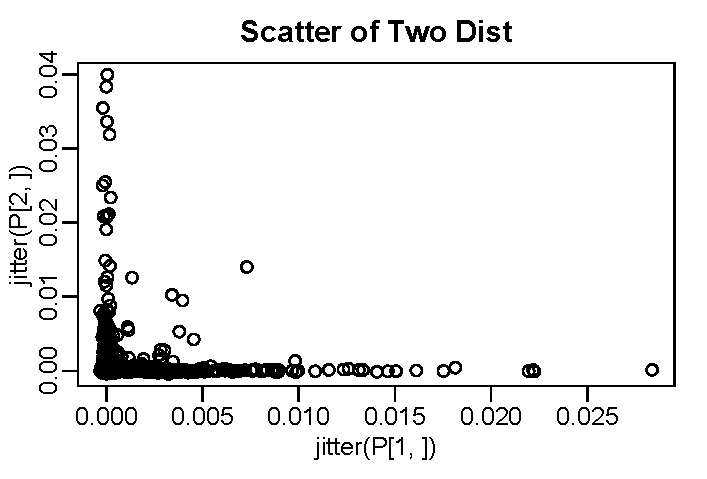
\includegraphics[width=3in]{figures/simdist}    
     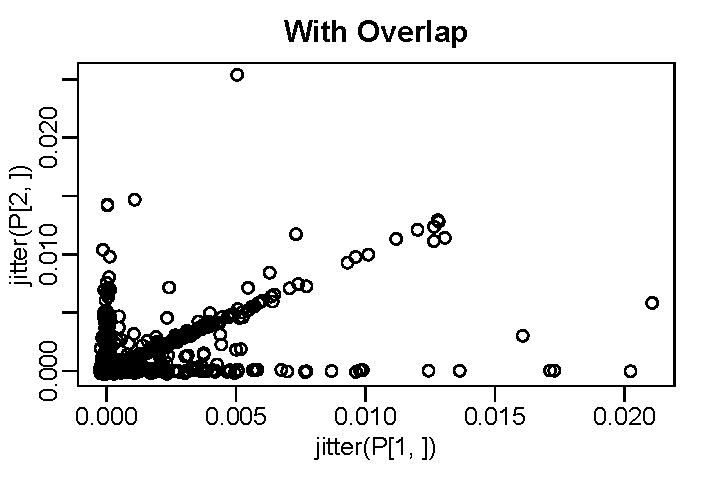
\includegraphics[width=3in]{figures/simdistB}    }
\end{figure}


The distribution of words produced by this topic model  loosely resembles the distribution found in real estate ads.  Compare Figure \ref{fig:simzipf}(a) to Figure \ref{fig:zipf} from the real estate data.  Though a good match for the less common words, the most common words are not as common as one might want.  The common words do not have a high enough frequency (disjoint topics lack common words like `a' and `the' and punctuation as found in the real-estate listings shown in Figure \ref{fig:zipf}), and the frequencies for rare words drop off too quickly.  


\begin{figure}
\caption{ \label{fig:simzipf} { \sl Distribution of word frequencies for simulated
topic data, based on (a) disjoint word distributions and (b) over-lapping distributions.}}
 \centerline{
 \vspace{0.1in}
 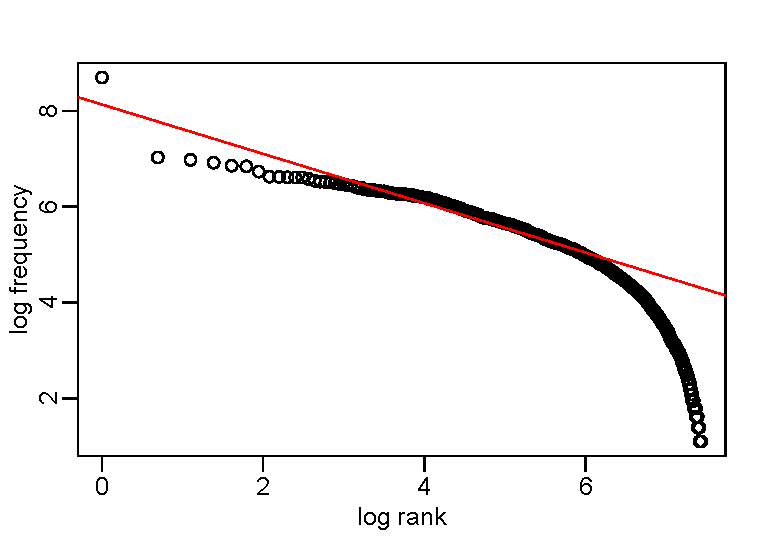
\includegraphics[width=2.5in]{figures/simzipfA}  
 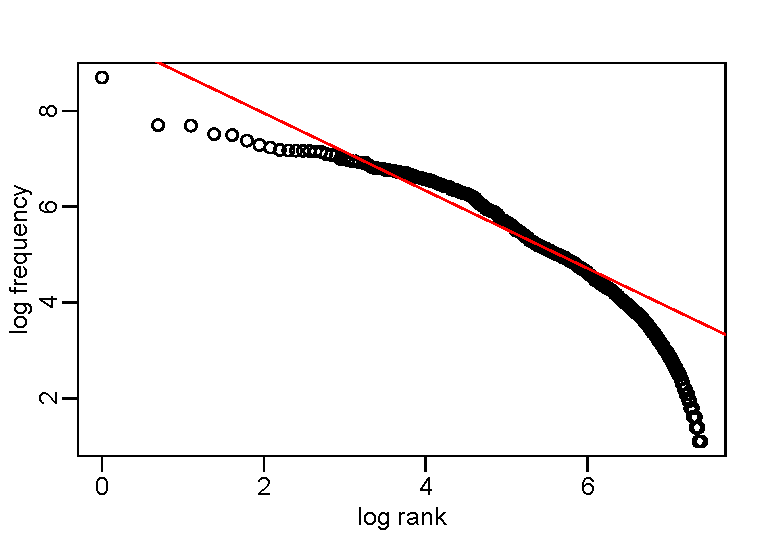
\includegraphics[width=2.5in]{figures/simzipfB} }
  \vspace{0.2in}
 \end{figure}


Table \ref{tab:simregr} summarizes the fits using $k_W = 100$ singular vectors and $k_B=100$ left and right singular vectors of $B$.  The fits recover much, but certainly not all of the underlying regression structure (for which $R^2 \approx 0.92$).  The fitted models produce similar fitted values, as shown in Figure \ref{fig:simfits}.  The two fits, however, deviate for documents with either lower or higher values of $y$. 

% \ras{ Would measurement error produce this tail curvature?}

\begin{table} 
\caption{ \label{tab:simregr}
\sl Fits to regression in simulated topic data using singular vectors of $W$ and $B$ for two topic distributions.}
\begin{center} 
\begin{tabular}{|c|ccc|}
\hline
  Topic Structure & Num Regressors & Origin & $\ol{R}^2$ \cr \hline \hline
   Disjoint            &         100              &  $W$  &  0.746        \cr
                           &         200              &  $B$  &   0.788        \cr \hline \hline
   Overlapping    &          100              &  $W$ &   0.516       \cr
                           &          200             &  $B$  &   0.626        \cr \hline
\end{tabular}
\end{center}
\end{table}


\begin{figure}
\caption{ \label{fig:simfits}  
{\sl Scatterplot of fitted values for the two regressions based on singular vectors of $W$ and $B$.}  The shown smooth curve is the lowess fit, and the correlation $r \approx 0.97$.}
\centerline{  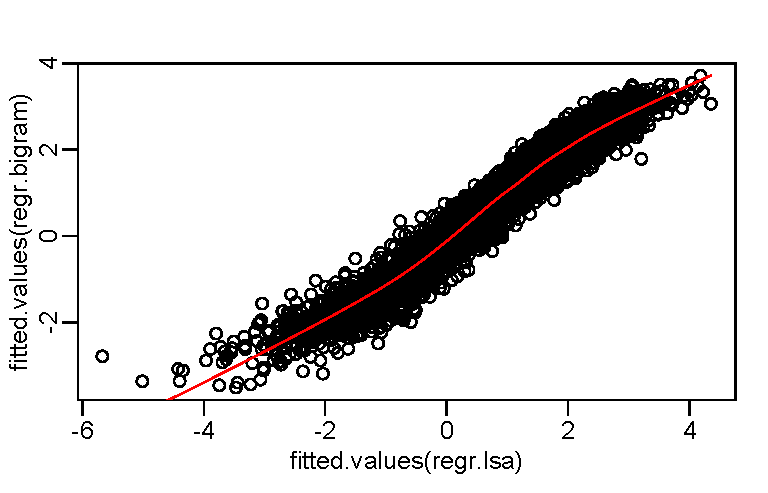
\includegraphics[width=4in]{figures/simfits}  }
\end{figure}


Because the topic distributions are nearly disjoint, one can identify the number of topics $K$ from the singular value decompositions.  The value of $K$ is most apparent in a canonical correlation analysis of the singular vectors of $B$.  Figure \ref{fig:simccab} graphs the canonical correlations for the left and right singular vectors
of the bigram matrix for the simulated text.  The clear break in the sequence of singular vectors confirms the presence of $K=10$ topics.  

 \begin{figure}
  \caption{ \label{fig:simccab} { \sl Canonical correlations for left and right
 singular vectors of the bigram matrix $B$ of simulated topic data.} (a) The underlying topics are nearly disjoint in support. (b) The underlying topics overlap.}
\vspace{0.1in}
 \centerline{
      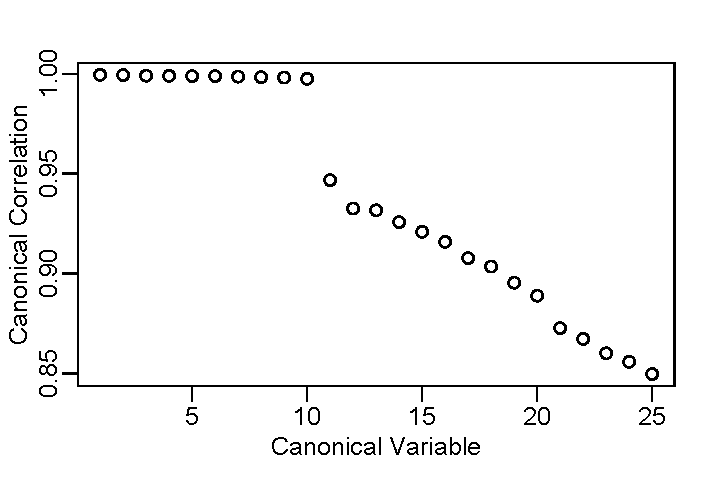
\includegraphics[width=3in]{figures/simccab}  
      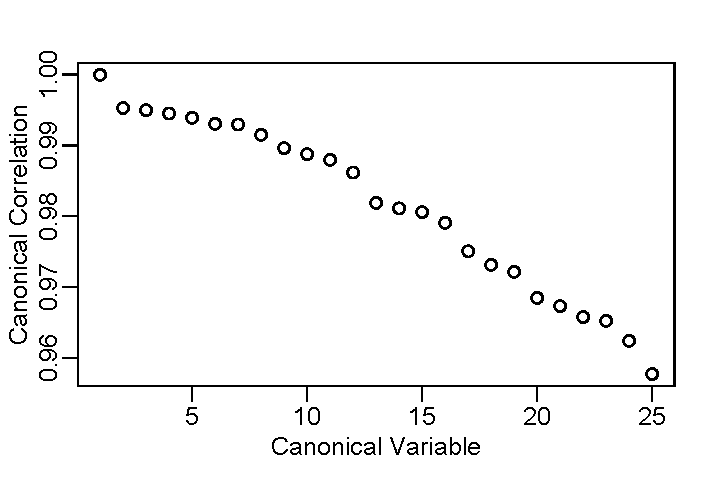
\includegraphics[width=3in]{figures/simccabb}   }
  \end{figure}
 
 
 \subsubsection{Overlapping Topic Distributions} % -----------------
 
 The ability to recover the underlying regression structure is diminished in the presence of overlapping topics.  The simulation in this section is virtually identical to the previous one, but for overlapping topics.  The simulation again has a vocabulary of $M=2,000$ words, $n=6,000$ documents, and $K=10$ topics.  Rather than simulate the topics distributions independently, however, we introduce a common structure.  The topic distributions share 150 ``common words'' that follow with probabilities from a Dirichlet distribution.  Let $X \sim \mbox{Dir}(150, 2)$ and let $\xi$ denote the vector obtained by concatenating $M$ - 150 zeros onto $X$, $\xi' = (X, 0 , \ldots, 0)$.  The distribution that defines the $k$th trait is then $P_k = \xi/2 + Z/2$ with $Z \sim \mbox{Dir}(\al_m)$.  Figure \ref{fig:simdist}(b) plots the probabilities of two distributions generated in this manner.  The diagonal points show the substantial overlap.  The number of topics per document and the marginal distribution of words per document are both similar to the prior simulation and are not materially influenced by the introduction of this overlap.
 
 
 The same cannot be said for the regressors produced from singular value decompositions.  The lower portion of Table \ref{tab:simregr} summarizes these fits.  The regression on 100 singular vectors from $W$ now captures $\ol{R}^2 = 0.516$ of the variation in the response, and the regressors from the bigram obtain $\ol{R}^2 = 0.626$.  The correlation between fitted values falls to 0.86 (down from 0.97 when no overlap was introduced).  Curiously, the bigram is less influenced by the overlap.  
 Canonical correlation of the singular vectors of $B$ also no longer reveals the number of topics (Figure \ref{fig:simccab}(b)).   The canonical correlations between left and right singular vectors of $B$ now provide no hint as to the choice of $K$.  
 
 
 Figure \ref{fig:simregr} summarizes the statistical significance of the coefficient estimates in this model.  The distribution of significance is rather different from that seen in the real estate models (Figure \ref{fig:svdregr}).  For example, statistical significance decays in the real estate model as one moves from the leading singular vectors of $W$ down to smaller vectors.  The simulated results show no hint of greater significance in the leading singular vectors and have a diffuse signal.
  Also, both half-normal plots are very nearly linear, with little of the ``superstar'' character seen in the $t$-statistics from the regression models for real estate.  What is similar to the model for prices is that the signal is more diffuse in the regression using correlation regressors derived from $B$.  The slope of the line fitted to the half-normal plot of the $t$-statistics for the singular vectors of $W$ is 8.8, whereas that for the regressors derived from $B$ is 3.6.  
 
 
 \begin{figure}
 \caption{ \label{fig:simregr}
  {\sl Distribution of statistical significance in the regression with simulated, overlapping topic models.} Results first for the regression on singular vectors from $W$, then those derived from the bigram matrix $B$.}
   \centerline{ 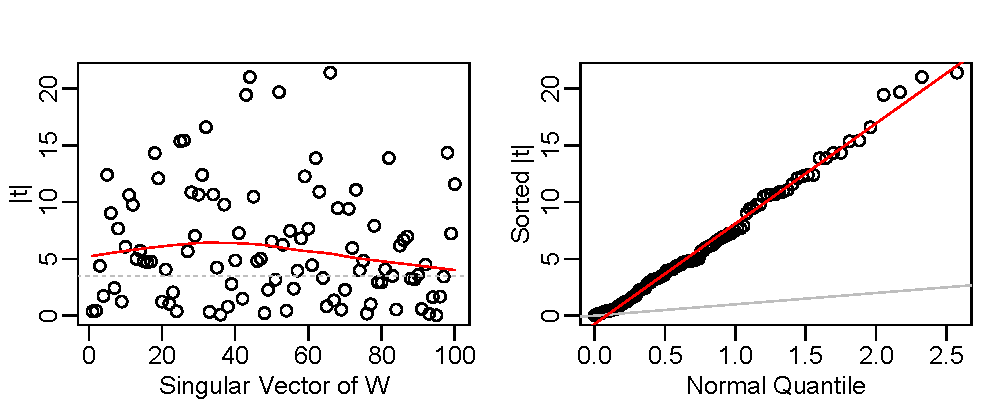
\includegraphics[width=5in]{figures/simregrW}  }
   \centerline{ 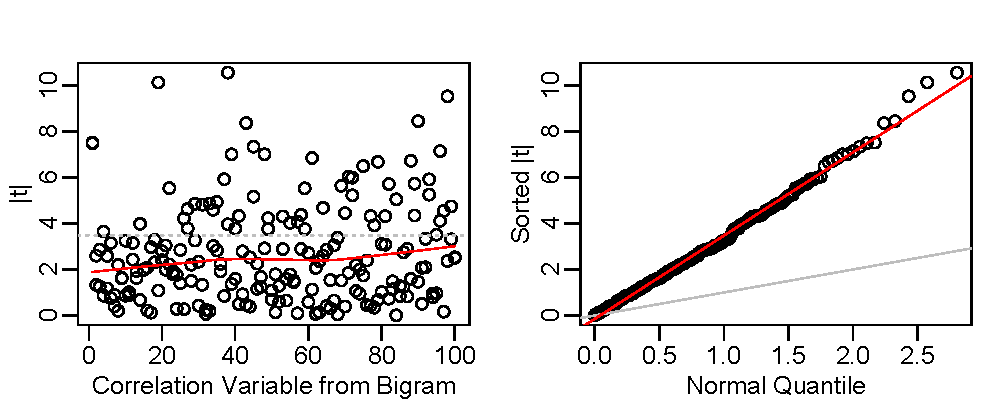
\includegraphics[width=5in]{figures/simregrB}  }
 \end{figure}

%--------------------------------------------------------------------------
\section{Variable Selection and Cross Validation}
\label{sec:cv}
%--------------------------------------------------------------------------

The previous examples routinely estimate regression models with hundreds of explanatory variables.  Though large by traditional standards, these models do not suffer from the problems associated with over fitting because we have not used the data to pick the model.  We simply fit a large collection of regressors.  Evaluating such models is thus the province of classical statistical tests and criteria such as adjusted r-squared.  

As evidence that these models are not over fit, we offer the following example.  Consider the LSA regression that uses 500 principal components of $W$.  Adjusting for the effects of estimating the 500 coefficients and the intercept anticipates the out-of-sample mean squared error of prediction to be $s_e^2 (1+(p+1)/n)$.  This simple approximation averages over the regression design, ignoring leverage effects.  Plugging in the unbiased estimate $s_e^2 = 0.5649$ gives $0.5649 (1+501/7384) = 0.603$.  Because the values of the regressors in the test data do not match those in the training data, this estimator is typically smaller than the observed MSE by an amount depending on variation in the regressors.  

For comparison, we performed repeated 10-fold transductive cross validation.  Transductive cross-validation presumes that the full collection of regressors is available for the training data, which in this case implies that we have all of the data available to perform the principal components analysis.  Only the values of the response are hidden in each fold of the cross-validation; the collection of regressors is fixed.  We repeated the 10-fold cross-validation 20 times, each time randomly partitioning the cases into 10 folds. The observed average squared error was slightly higher than anticipated at $0.614 \pm 0.007$, but basically agreed with the estimate from the fitted model. 


%--------------------------------------------------------------------------
\section{Lighthouse Variables and Interpretation}
\label{sec:light}
%--------------------------------------------------------------------------
 
 

 Our emphasis on predictive accuracy does not necessarily produce an
 interpretable model, and one can use other data to create such structure.  Our
 explanatory variable resemble those from principal components analysis and
 share their anonymity.  To provide more interpretable regressors, the presence
 of partial quantitative information in real estate listings (\eg, some listings
 include the number of square feet) provides what we call ‘lighthouse variables’
 that can be used to derive more interpretable variables.  In our sample, few
 listings (about 6\%) indicate the number of square feet.  With so much missing
 data, this manually derived predictor is not very useful as an explanatory
 variable in a regression.  This partially observed variable can then be used to
 define a weighted sum of the anonymous text-derived features, producing a
 regressor that is both complete (no missing cases) and interpretable.  One
 could similarly use features from a lexicon to provide more interpretable
 features.


Though regression models are seldom causal, one is often tempted to interpret
 properties of the solution within the domain of application.  Because the
 predictors computed from the decompositions in the prior section describe
 subspaces rather than some specific property of words, interpretation is
 essentially non-existent.


 To obtain features that are interpretable, we exploit the pre<sence of
 characteristics that are occasionally observable.  For example,
 most home listings do not include the number of bathrooms.  An
 explanatory variable obtained by parsing this count is missing for 74\% of the property listings.  We can use this partially observed variable, however, to construct a more interpretable variable from either the principal components of $W$ or the bigram variables.  


 Let $z \in \Rn$ denote the partially observed or perhaps noisy data
 that measures a substantively interesting characteristic of the
 observations.  For our example, $z$ is the partially observed count of the number of bathrooms.  Rather than use $z$ directly as a predictor of $y$, we
 can use it to form an interpretable blend of, for instance, $U_W$.   In
 particular, we simply regress $z$ on these columns, finding the
 linear combination of these basis vectors most correlated with the
 observed variable.  This variable, call it $\hat{z}$ then becomes
 another regressor.  Because such variables can be used to guide the
 construction of interpretable combinations of the bases $U_W$ and
 $C$, we call these lighthouse variables.  
 
 
 In our example, the correlation between the number of bathrooms and the price of the listing is 0.42 for listings that show this characteristic.  This correlation is much smaller (0.19) if we fill the missing values with the mean number of bathrooms (Figure  \ref{fig:parsed}).  If we form the projection $\hat{z}$ given by regressing the observed counts on the corresponding rows of $U_W$, this new regressor has correlation 0.29 with the log of price.



%--------------------------------------------------------------------------
\section{Summary and Next Steps}
\label{sec:disc}
%--------------------------------------------------------------------------
  
  Regression modeling always benefits from greater substantive insight, and the modeling of text is no exception.  An obvious approach to building regressors from text data relies on a
 substantive analysis of the text.  For example, sentiment analysis constructs a
 domain-specific lexicon of positive and negative words.  In the context of real
 estate, one might suspect  words such as ``modern'' and ``spacious''  to be associated with more expensive properties, whereas
 ``Fannie Mae'' and ``fixer-upper'' to signal properties with lower prices.  The
 development of such lexicons has been an active area of research in sentiment
 analysis over the past decade \citep{taboada11}.  The development of a lexicon
 require substantial knowledge of the context and the results are known to be
 domain specific.  Each new problem requires a new lexicon.  The lexicon for
 pricing homes would be quite different from the lexicon for diagnosing patient
 health.  Our approach is also domain specific, but requires little user input
 and so can be highly automated.


 Our analysis here shows that one can exploit well-known methods of multivariate analysis to create regressors from unstructured text.  Compared to iterative methods based on MCMC, the computations are essentially immediate.  Surprisingly, the resulting regressors are quite predictive in several examples we have explored.  For example, we used this same methodology to model ratings assigned to wines based on tasting notes.  The tasting notes themselves are typically shorter than these real estate listings (averaging about 42 tokens compared to 72 for the listings), but we have a larger collection of about 21,000.  Using the methods demonstrated here, a regression using 250 principal components of $W$ explains about 66\% of the variation in ratings, we a remarkably similar distribution of effect sizes as shown in Figure \ref{fig:wine}.  Similarly, regression on the 250 left and 250 right regressors constructed from the bigram matrix explains about 68\% of the variation.  We plan to explore other applications in the near future.
 
 
 \begin{figure}
 \caption{ \label{fig:wine} \sl Regression t-statistics from a model that predicts wine ratings using 250 principal components of $W$ based on 21,000 wine tasting notes.}
 
 \centerline{
   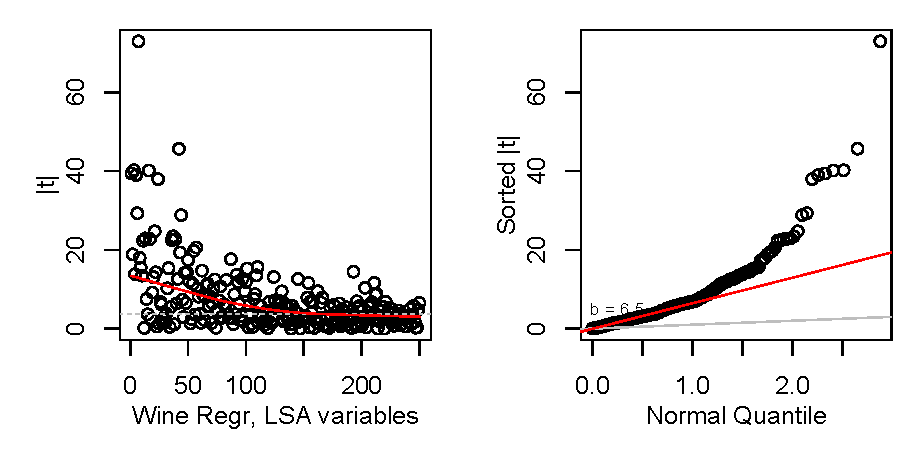
\includegraphics[width=4in]{figures/wine.pdf}
   }
  \end{figure} 
  
  
   The connection to topic models is an important aspect of these results.  Topic models define a DGP for which the regressors that we construct capture the underlying data-generating mechanism.  If one accepts topic models as a reasonable working model of the semantics of text, then it is no accident that regressors constructed from text are predictive.


 Our work here merely introduces these methods, and we hope that this introduction will encourage more statisticians to engage problems in  modeling text.  Our results here also suggest several directions for further research:

   \begin{description}
   
   \item[n-grams.]  Our example uses bigrams to capture word associations captured by adjacent placement.  Other reasonable choices define different measures of context,  such as trigrams (sequence of 3 words) or skipped bigrams (words separated by some count of tokens).  Some preliminary results show, for instance, that trigrams offer modest gains, albeit at a nontrivial increase in computation.
   
   \item[Transfer learning.]  Transfer learning refers to learning what can be extrapolated from one situation to another.  In our context, it would be of interest to learn how well models developed from data in June 2013 work when applied to data from later time periods or different locations.  It is evident that the models shown here would not perform so well applied to the language of a different market, such as in Miami or Los Angeles.  Not only do the characteristics of valuable properties change, but  local conventions for phrasing listings are also likely to be different.  Having a methodology for distinguishing idiosyncratic local features from those that generalize in time or space would be valuable. 
   
  \item[Alternative forms of tokenization.] Would be interesting to explore the use of stemming to reduce the number of word types and with a larger collection of documents, to explore annotation (that would distinguish words by their part of speech).  Further parsing, lexical analysis.  Some readers will be troubled by the simplicity of the  bag-of-words representation of a document.  Our methods understand neither the English language nor the rules of grammar and spelling.  They do not attempt to untangle  multiple uses of the same word.  Linguists have debated the ability of such  representations to reveal the meaning of language, and it is clear that the bag of words representation loses information.  Just imagine cooking from``bag of words'' recipe or following a ``bag of words'' driving directions.  Nonetheless, this very direct representation produces very useful explanatory variables within our application.  We leave open the opportunity to embellish this approach with more domain specific methods of parsing, such as adding part-of-speech tags and lexical information.
   
   \item[Use of unsupervised data.] Most words are used only once or twice, meaning that we lack enough data to identify their connection to the response or indeed to other words.  As a partial remedy, it may be possible to build regressors that represent such words from larger, more generic text such as the collection of n-grams collected by Google.  Using this supplemental unsupervised data requires solving the problem of transfer learning, at least to some degree, but opens the door to much more extensive examples. 
   
   \item[Variable selection.]  The distribution of effects (such as shown by the $|t|$ statistics of the text-derived regressors) are poorly matched to the so-called `nearly black' model commonly adopted in research on the theory of variable selection.  Rather than have most of the predictive power concentrated in a very small number of regressors, these regressors spread the power of many.  
   
   It would also be interesting to explore these models for nonlinearity. Variable selection is perhaps unnecessary for using the regressors derived from $U_W$ and $C$, but essential if one hopes to detect and incorporate nonlinearity. In particular, searching for nonlinearity -- such as interactions -- requires variable selection.  Even a very large corpus of documents looks small compared to the number of possible second-order interactions.  Finally, the ordered presentation of the $|t|$ statistics suggests an opportunity for variable selection derived from alpha investing \citep{fosterstine08}.  Alpha investing is a procedure for testing a sequence of hypotheses that benefits from {\it a priori} ordering of the tests.
   
   \end{description}

One can generalize LSA from words and documents to collections of other items,
 such as phonemes in speech or tones in music \cite[called latent semantic
 mappingin][]{bellegarda05}.



%--------------------------------------------------------------------------
\section*{Acknowledgement}
%--------------------------------------------------------------------------

The authors thank Vanessa Villatoro from Trulia's PR Team for allowing us to scrape the data from their web site.


%--------------------------------------------------------------------------
% References
%--------------------------------------------------------------------------

\bibliography{../../../references/stat,../../../references/TextPapers/text}
\bibliographystyle{../bst/ims}

\end{document} %==========================================================
